% !TEX encoding = UTF-8 Unicode
% !TEX root = DesignDocument.tex

\documentclass{book}

\usepackage{float}

% !TEX root = SystemTemplate.tex

\usepackage[width=6.5in, height=9.2in, top=1.0in, papersize={8.5in,11in}]{geometry}
\usepackage[pdftex]{graphicx}
\usepackage{amsmath}
\usepackage{amsthm}
\usepackage{amssymb}
%\usepackage{txfonts}
\usepackage{textcomp}
\usepackage{amsthm}
%\usepackage{minted}
\usepackage[all]{xy}
\usepackage{fancyhdr}
\pagestyle{fancy}
\usepackage{hyperref}
\usepackage{verbatim}
\usepackage{algorithm}
\usepackage{algorithmic}
\usepackage{array}
\usepackage{color}
\usepackage{listings}
\usepackage{calc}
\usepackage{doxygen}
\usepackage[utf8]{inputenc}
\usepackage{makeidx}
\usepackage{multicol}
\usepackage{multirow}
\usepackage[table]{xcolor}
\usepackage{tabularx}
\usepackage{framed}
\usepackage{xspace}
\usepackage{etex}
\usepackage{todonotes}
\usepackage{pdfpages}
\usepackage{pgfgantt}


%% Computer Modern Bright Font
%\usepackage{cmbright}
%\usepackage[T1]{fontenc}

%% Sans Serif Modern Font - similar to  Helvetica
\usepackage{lmodern}
\renewcommand*\familydefault{\sfdefault} %% Only if the base font of the document is to be sans serif
\usepackage[T1]{fontenc}


\definecolor{SDColor1}{rgb}{0,0,0}
\definecolor{SDColor2}{rgb}{0,0,0}
\definecolor{SDColor3}{rgb}{0,0,0}
\definecolor{SDColor4}{rgb}{0,0,0}
\definecolor{SDColor5}{rgb}{0,0,0}

%%%  --- Here are some other colors.  Keep it conservative --- %%%

%% Blue font color scheme
%\definecolor{SDColor1}{rgb}{.204,.353,.541}
%\definecolor{SDColor2}{rgb}{.31,.506,.741}
%\definecolor{SDColor3}{rgb}{0.18,0.35,0.59}
%\definecolor{SDColor4}{rgb}{0.44,0.59,0.82}
%\definecolor{SDColor5}{rgb}{0.35,0.35,0.35}
%

%% Brown color scheme
% \definecolor{SDColor1}{rgb}{.55,.2,.2}
%\definecolor{SDColor2}{rgb}{.4,.1,.1}
%\definecolor{SDColor3}{rgb}{.5, .15,.15}
%\definecolor{SDColor4}{rgb}{.63,.32,.18}
%\definecolor{SDColor5}{rgb}{.45,.15,.15}
%


%% Custom colors for code listing environment
\definecolor{OliveGreen}{cmyk}{0.64,0,0.95,0.40}
\definecolor{DarkBlue}{cmyk}{0.76,0.76,0,0.20}
\definecolor{DarkRed}{cmyk}{0,1,1,0.45}
\lstset{language=c,frame=ltrb,framesep=5pt,basicstyle=\normalsize,
 keywordstyle=\ttfamily\color{DarkRed},
identifierstyle=\ttfamily\color{DarkBlue}\bfseries,
commentstyle=\color{OliveGreen},
stringstyle=\ttfamily,
showstringspaces=false,tabsize = 3}


\setlength{\oddsidemargin}{0mm} 
\setlength{\evensidemargin}{0mm} 

%% Uncomment if you want "Draft" placed on each page.
%\usepackage{draftwatermark}
%\SetWatermarkLightness{0.975}
%\SetWatermarkScale{1}
%\SetWatermarkText{Draft}

\pagestyle{fancy}
\renewcommand{\chaptermark}[1]{\markboth{#1}{}}
\renewcommand{\sectionmark}[1]{\markright{\thesection\ #1}}
\fancyhf{}
\fancyhead[LE,RO]{\bfseries\thepage}
\fancyhead[LO]{\bfseries\rightmark}
\fancyhead[RE]{\bfseries\leftmark}
%\fancyfoot[LE,RO]{Confidential and Proprietary}
%\renewcommand{\headrulewidth}{0.5pt}
%\renewcommand{\footrulewidth}{0pt}
%\addtolength{\headheight}{0.5pt}
%\setlength{\footskip}{0mm}
%\renewcommand{\footruleskip}{0pt}



\usepackage{titlesec}
\titleformat{\chapter}[display]
{\normalfont\bfseries\color{SDColor3}}    %\normalfont\bfseries\filcenter}
{\LARGE\thechapter}
{1ex}
{\titlerule[2pt]
\vspace{2ex}%
\LARGE}
[\vspace{1ex}%
{\titlerule[2pt]}]

%
%\usepackage{titlesec}
%\titleformat{\chapter}{\normalfont\bfseries\LARGE}
%{\thechapter.}{5pt}{}[{\titlerule[3pt]}]
%
%\titleformat{\section}{\normalfont\bfseries\Large}
%{\thesection.}{5pt}{}[{\titlerule[2pt]}]
%
%\titleformat{\subsection}{\normalfont\bfseries\large}
%{\thesubsection.}{5pt}{}[{\titlerule[1pt]}]
%


%\titleformat*{\section}{\Large\bfseries\sffamily\color{SDColor1}}
%\titleformat*{\subsection}{\large\bfseries\sffamily\color{MSLightBlue}}
%\titleformat*{\section}{\Large\bfseries\color{SDColor3}}
%\titleformat*{\subsection}{\large\bfseries\color{SDColor4}}

%\titleformat*{\section}{\Large\bfseries}
%\titleformat*{\subsection}{\large\bfseries}
%\titleformat*{\subsubsection}{\large\bfseries}

\titleformat*{\section}{\Large\bfseries\color{SDColor1}}  
\titleformat*{\subsection}{\large\bfseries\color{SDColor2}}
\titleformat*{\subsubsection}{\large\bfseries\color{SDColor5}}
\setcounter{secnumdepth}{3}
\renewcommand{\thesubsubsection}{\thesubsection.\alph{subsubsection}}

% Save the original chapter command as stdchapter
\let\stdchapter\chapter

%redefine the backmatter command
\let\stdbackmatter\backmatter
\makeatletter% We need the '@' letter to call if@openright
\renewcommand{\backmatter}{
\stdbackmatter
% need to set the page counter back to 1
\setcounter{page}{1}
%% Redefine the \chapter command for our Back Matter
\renewcommand{\chapter}[1]{
  \if@openright\cleardoublepage\else\clearpage\fi% chapters begin on right page
  \stdchapter{##1}% output standard chapter heading
  \setcounter{section}{0}% restart the section numbering
  \renewcommand{\thepage}{BM-\arabic{page}}% Redefine page numbering format
  \renewcommand{\thesection}{\arabic{section}}% Redefine section number format
}}
\makeatother% Restore the normal behavior of '@'

%redefine the appendix command
\let\stdappendix\appendix
\makeatletter% We need the '@' letter to call if@openright
\renewcommand{\appendix}{
\stdappendix
%% \titleformat{\chapter}[display]
%% {\normalfont\bfseries\color{SDColor3}}    %\normalfont\bfseries\filcenter}
%% {\LARGE Appendix \thechapter}
%% {1ex}
%% {\titlerule[2pt]
%% \vspace{2ex}%
%% \LARGE}
%% [\vspace{1ex}%
%% {\titlerule[2pt]}]
  %%% Since counters are different in the appendix section
  %%% we redefine \chapter to explicitly reset the page number
  %%%  (comment out to see effect)
  \renewcommand{\chapter}[1]{
    \stdchapter{##1}\setcounter{page}{1}
    %%% We also redefine page numbering
    \renewcommand{\thepage}{\Alph{chapter}-\arabic{page}}
  }
}
\makeatother% Restore the normal behavior of '@'


\makeatletter% We need the '@' letter to call if@openright
\newcommand{\agreement}{
  \renewcommand{\chapter}[1]{
    \if@openright\cleardoublepage\else\clearpage\fi% chapters begin on right page
    \pagestyle{plain}% turn off fancy headers
    \setcounter{section}{0}% Reset the section number
    \setcounter{page}{1}% Reset the page number
    \renewcommand{\thepage}{SA-\arabic{page}}% Set format for page numbering
    \renewcommand{\thesection}{\arabic{section}}% Set format for section numbering
    \refstepcounter{chapter}% Add it to the index/toc for on-line viewing
    \addcontentsline{toc}{chapter}{##1}% Add to the table of contents
  }
}
\makeatother% Restore the normal behavior of '@'



%%  If you do some math typesetting, you may want more environment names.
%% Uncomment to see how this works:
%\newtheorem{summary}{Summary:}
%\newtheorem{example}{Example:}



 % This sets the format.

% Add your title page contents here 
\title{{\color{SDColor3} \rule{\linewidth}{0.5mm}}\\[2mm] {\huge \bfseries \color{SDColor3} ARM Cluster }\\[-1mm] {\color{SDColor3}\rule{\linewidth}{0.5mm}} \\  \vfill
{\LARGE \bfseries \color{SDColor4} Senior Design Final Documentation }\\  \vfill 
{\color{SDColor3} Discoverment} }
\author{\color{SDColor3}  Andrew Kenneth Hoover \and \color{SDColor3} Christine Norma Sorensen }
\date{\color{SDColor3} \today}


\begin{document}

\frontmatter

\addcontentsline{toc}{chapter}{Title}
\maketitle
\tableofcontents
\addcontentsline{toc}{chapter}{Contents}
\listoffigures
%%\addcontentsline{toc}{chapter}{List of Figures}
%%\listoftables
%%\addcontentsline{toc}{chapter}{List of Tables}
%%\listofalgorithms
%%\addcontentsline{toc}{chapter}{List of Algorithms}

\chapter{Overview Statements}
% !TEX root = DesignDocument.tex

\section{Mission Statement}
To create the fastest, most effcient cluster of single-board computers.

\section{Elevator Pitch}
Our goal is to build a cluster of single-board computers that produces as many floating-point operations possible per watt per dollar. We are testing three computers:  ODROID, Raspberry Pi, and PcDuino and finding alternative modes of communication outside of the traditional ethernet port in order to find what best fits our cluster.
  % add mission statement to mission.tex

\chapter{Document Preparation and Updates}
%old
% !TEX root = SystemTemplate.tex



Current Version [3.2.0]
\vspace*{5mm}

{\color{MSBlue3}
\noindent
\textit{Prepared By:}\\
\textit{Andrew Hoover}\\
\textit{Christine Sorensen}
}

\vfill
\noindent
{\color{color02} \textit{\textbf{Revision History}}}\\
\begin{tabular}{|>{\raggedright}p{1.5cm}|>{\raggedright}p{3cm}|>{\raggedright}p{1.5cm}|>{\raggedright}p{9cm}|}
\hline
\textit{\textbf{Date}} &  \textit{\textbf{Author}} & \textit{\textbf{Version}} & \textit{\textbf{Comments}}\tabularnewline
\hline
\textit{\textbf{09/14/15}} & \textit{Christine Sorensen} & \textit{1.0.0} & \textit{Initial version}\tabularnewline
\hline
\textit{\textbf{10/02/15}} & \textit{Christine Sorensen} & \textit{1.1.0} & \textit{Completion of Sprint \# 1}\tabularnewline
\hline
\textit{\textbf{11/09/15}} & \textit{Christine Sorensen} & \textit{2.0.0} & \textit{Updated Project Overview}\tabularnewline
\hline
\textit{\textbf{11/09/15}} & \textit{Christine Sorensen} & \textit{2.1.0} & \textit{Completion of Sprint \# 2}\tabularnewline
\hline
\textit{\textbf{12/09/15}} & \textit{Christine Sorensen} & \textit{3.0.0} & \textit{Completion of Sprint \# 3}\tabularnewline
\hline
\textit{\textbf{12/10/15}} & \textit{Andrew Hoover} & \textit{3.1.0} & \textit{Design and implementation and Unit Testing documentation}\tabularnewline
\hline
\textit{\textbf{12/11/15}} & \textit{Christine Sorensen} & \textit{3.2.0} & \textit{Added to log entries. Added resumes.}\tabularnewline
%%Use this to add an entry
%%\hline
%%\textit{\textbf{3/4/12}} & \textit{Team Member \#3} & \textit{1.1.0} & \textit{Edited version}\tabularnewline
 \hline
 &  &  & \tabularnewline
\hline
 &  &  & \tabularnewline
\hline
 &  &  & \tabularnewline
\hline
 &  &  & \tabularnewline
\hline
\end{tabular}
\vfill


 
\mainmatter

%% The term "cleaning" used in the syllabus means removing all of the sample content I
%% have provided.   You can comment out by using the comment character or the comment
%% environment.  

%%  Add to the following chapters

% !TEX root = SystemTemplate.tex

\chapter{Overview and concept of operations}

*The overview should take the form of an executive summary.  Give the reader a feel 
for the purpose of the document, what is contained in the document, and an idea 
of the purpose for the system or product. 


\section{Scope}
*What scope does this document cover? 

\section{Deliverables}
\begin{itemize}
	\item ARM Cluster
	\item Research Symposium
	\item Design Fair
	\item Documentation
\end{itemize}

\section{Purpose}
The purpose of this project is to build a cluster of 6-12 single-board computers. This cluster should perform floating-point operations. With research, the cluster will have a new mode of communication and be able.

\subsection{Major System Component \#1}
*Describe briefly the role this major component plays in this system. 

\subsection{Major System Component \#2}
*Describe briefly the role this major component plays in this system. 

\subsection{Major System Component \#3}
*Describe briefly the role this major component plays in this system. 

\section{Systems Goals}
*Briefly describe the overall goals this system plans to achieve.
*These goals are typically provided by the stakeholders.  This is not
intended to be a detailed requirements listing.  Keep in mind that
this section is still part of the Overview.

\section{System Overview and Diagram}
*Provide a more detailed description of the major system components
without getting too detailed.  This section should contain a
high-level block and/or flow diagram of the system highlighting the
major components.  See Figure~\ref{systemdiagram}.  This is a floating
figure environment.  \LaTeX\ will try to put it close to where it was
typeset but will not allow the figure to be split if moving it can not
happen.  Figures, tables, algorithms and many other floating
environments are automatically numbered and placed in the appropriate
type of table of contents.  You can move these and the numbers will
update correctly.

\begin{figure}[tbh]
\begin{center}
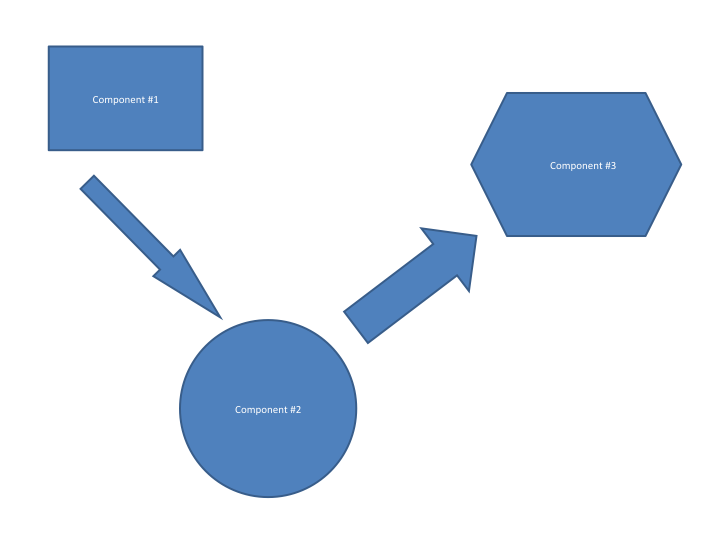
\includegraphics[width=0.75\textwidth]{./diagram}
\end{center}
\caption{A sample figure .... System Diagram \label{systemdiagram}}
\end{figure}

\section{Technologies Overview}
*This section should contain a list of specific technologies used to
develop the system.  The list should contain the name of the
technology, brief description, link to reference material for further
understanding, and briefly how/where/why it was used in the system.
See Table~\ref{somenumbers}.  This is a floating table environment.
\LaTeX\ will try to put it close to where it was typeset but will not
allow the table to be split.

\begin{table}[tbh]
\caption{A sample Table ... some numbers. \label{somenumbers}}
\begin{center}
\begin{tabular}{|r|l|}
  \hline
  7C0 & hexadecimal \\
  3700 & octal \\ \cline{2-2}
  11111000000 & binary \\
  \hline \hline
  1984 & decimal \\
  \hline
\end{tabular}
\end{center}
\end{table}

  %% All tracks
% !TEX root = SystemTemplate.tex
\chapter{User Stories, Backlog and Requirements}
\section{Overview}


The overview should take the form of an executive summary.  Give the reader a feel 
for the purpose of the document, what is contained in the document, and an idea 
of the purpose for the system or product. 

 The userstories 
are provided by the stakeholders.  You will create he backlogs and the requirements, and document here.  
This chapter should contain 
details about each of the requirements and how the requirements are or will be 
satisfied in the design and implementation of the system.

Below:   list, describe, and define the requirements in this chapter.  
There could be any number of sub-sections to help provide the necessary level of 
detail. 





\subsection{Scope}


What scope does this document cover?  This document would contain stakeholder information, 
initial user stories, requirements, proof of concept results, and various research 
task results. 



\subsection{Purpose of the System}
The system is used for research purposes and a proof of concept. 


\section{ Stakeholder Information}
One stakeholder is Dr. Christer Karlsson. If this project is successfully completed,
Dr. Karlsson plans to use the research and project results as a proof of concept. 


\subsection{Customer or End User (Product Owner)}
Dr. Christer Karlsson is the end user.  The end user might include 

Who?  What role will they play in the project?  Will this person or group manage 
and prioritize the product backlog?  Who will they interact with on the team to 
drive product backlog priorities if not done directly? 

\subsection{Management or Instructor (Scrum Master)}
Dr. Karlsson manages this project and drives the meetings.


\subsection{Investors}
Dr. Karlsson is the investor on the project. His role is also the client.

\subsection{Developers --Testers}
Andrew Hoover, Samantha Kranstz, and Christine Sorensen developed and tested 
the cluster. 


\section{Business Need}
There is no buisness need. This project solely for research purposes.  


\subsection{System  Requirements}
The only system requirement would be the cluster must be made of single-board
computers.


\subsection{Network Requirements}
Create a new network for the cluster.


\subsection{Development Environment Requirements}
None. 


\subsection{Project  Management Methodology}
Oral progress reports are due on Tuesdays and Thursdays at one o'clock in the 
afternoon. These reports are given to Dr. Karlsson. 
 
\begin{itemize}
\item Trello is used to manage the backlog and status.
\item All parties have access to the sprint and product backlogs.
\item Six sprints will be completed this project
\item The sprint cycles are a couple weeks long.
\item No restrictions on source control.
\end{itemize}

\section{User Stories}
This section can really be seen as the guts of the document.  This section should 
be the result of discussions with the stakeholders with regard to the actual functional 
requirements of the software.  It is the user stories that will be used in the 
work breakdown structure to build tasks to fill the product backlog for implementation 
through the sprints.

This section should contain sub-sections to define and potentially provide a breakdown 
of larger user stories into smaller user stories. 

\subsection{User Story \#1}
As a user, I want a cluster of at least 6 and no more than 12 single-board computers.
\subsubsection{User Story \#1 Breakdown}
The cluster will be made of ODROIDs, PcDuinos, or Raspberry Pi's, depending on which performs best in the benchmark tests.

\subsection{User Story \#2} 
As a user, I want the fasest, most efficient in both cost and operation cluster.
\subsubsection{User Story \#2 Breakdown}
Testing will be done on the single-board computers compared with prices to determine which will be best for the ARM cluster.

\subsection{User Story \#3} 
I want to the cluster to be at or below the maximum budget of \$1,200.00.
\subsubsection{User Story \#3 Breakdown}
The budget must include all components of the cluster: the computer boards, cost of power, switch, memory, cables, and power strips.

\subsection{User Story \#4}
I want to know which of the single-board computers is the fastest in GFlops/\$/Watt.
\subsubsection{User Story \#4 Breakdown}
Testing will take place on the ODROID, PcDuino, and Raspberry Pi to determine which is the fastest in this metric. 

\subsection{User Story \#5} 
I want a different communication mode beyond standard Ethernet.
\subsubsection{User Story \#5 Breakdown}
Utilize the other pins and ports to find an alternative form of communication.

\subsection{User Story \#6} 
Develop a message passing protocol for the communication.
\subsubsection{User Story \#6 Breakdown}
There is no message passing protocol for the other modes of communication. They must be developed and benchmarked.

\section{Research or Proof of Concept Results}
This project will be used as a proof of concept.
  %% All tracks (minimal for research track)
% !TEX root = SystemTemplate.tex


\chapter{Project Overview}
%*This section provides some housekeeping type of information with regard to the 
%team, project, etc. 



\section{Team Members and Roles}
\begin{itemize}
	\item Andrew Hoover - hardware/testing/software
	\item Samantha Kranstz - 
	\item Christine Sorensen - team lead/parallel programmer/software
\end{itemize}

\section{Project  Management Approach}
Project will be split into six sprints, each lasting two weeks. Items from the backlog are organized and assigned into these sprints. \newline \newline Product backlog is located on the Trello board. Documents and source code is located on Github. \newline \newline Formal meetings take place twice a week on Tuesdays and Thursdays at 1:00pm in advisor's, Dr. C. Karlsson's, office. Casual meetings are planned as needed.

\section{Phase  Overview}


%%If the system will be implemented in phases, describe those phases/sub-phases (design, 
%%implementation, testing, delivery) and the various milestones in this section. 
 %%This section should also contain a correlation between the phases of development 
%%and the associated versioning of the system, i.e. major version, minor version, 
%%revision. 

\section{Terminology and Acronyms}
\begin{itemize}
	\item Benchmarking - running tests in order to assess the perfomance of the computers
	\item iperf - tool in standard Debian repositories to test network speed
\end{itemize}


%%*Provide a list of terms used in the document that warrant definition.  Consider 
%%industry or domain specific terms and acronyms as well as system specific. 
   %% All tracks
% !TEX root = SystemTemplate.tex

\chapter{Design  and Implementation}

The design of the cluster is going change as we test different configurations to determine which is capable of producing the most gigaflops, and as we test different connection methods as we design our custom data transfer protocol. This section will outline the different designs we have created, how they were implemented, and our plans for implementing future designs going forward.
 

\section{Cluster Configure}

The first design we implemented was a star topology, with each device of the eight devices connected over Ethernet to a central switch. Each device was configured to be on the same network and capable of communicating over the switch via IP addresses. We configured the /home directory of our head node, Snow White, to be an NFS export that the seven other nodes would mount in their /home directory. 

\subsection{Technologies  Used}
We used several Linux system configuration tools to implement the cluster. We used the files
\begin{itemize}
	\item etc/network/interfaces
	\item etc/exports
	\item etc/hostname
	\item etc/hosts
	\item etc/fstab
\end{itemize}
for several different configuration setting. We also used a few packages availible from the defual debian repositories.
\begin{itemize}
	\item nfs-kernel-server
	\item nfs-common
	\item mpi-dev
\end{itemize}

Finally, we used SSH tools that are installed by default on Ubuntu 15.

\subsection{Component  Overview}
The features implented by this configuration were:

\begin{itemize}
	\item All devices recognizing the others over Ethernet.
	\item SSH without requiring a password.
	\item Mount home directory of Snow White on the dwarfs.
	\item Running MPI code on all devices.
\end{itemize}

\subsection{Phase Overview}
This is an extension of the Phase Overview above, but specific to this component. 
 It is meant to be basically a brief list with space for marking the phase status. 

\subsection{ Architecture  Diagram}
It is important to build and maintain an architecture diagram.  However, it may 
be that a component is best described visually with a data flow diagram. 

\subsection{Design Details}
First, we made the devices able to communicate on the same network. We assigned each device a static IP address by editing the /etc/networking/interfaces file to incluce the IP address chosen for the device. All addresses were on the 192.168.1.1 network, and the last number was 11 through 18 for the eight devices.

Next, we set each device to be able to use our naming convention in place of an IP address for any purpose, such as by using "ssh sleepy" instead of "ssh 192.168.1.13". To do this, we changed the /etc/hostname file to replace "odroid" with the name we wanted, and added entries to /etc/hosts to include the IP address of the other seven decives. 

We then set the /home directory of Snow White to be an NFS share that could be mounted on the dwarfs. After nfs-kernel-server was installed on Snow White, we edited it's /etc/exports file to include /home as an export. The dwarfs then installed nfs-common and used the command "mount SnowWhite:/home /home" to mount the home directory of Snow White over their own.

To make this mount process automatic on boot, we edited the /etc/fstab file on each dwarf to make them mount Snow White's home directory as part of the boot process. This proved unsuccesful, however, on all devices except for on. As a work around, we wrote a Python tool that can be run from Snow White to mount it's home directory on the dwarfs.


\begin{lstlisting}
#!/bin/usr/python

import os

def Main():

        hosts = [ 'snow_white', 'dopey', 'sleepy', 'grumpy', 'doc', 'happy',
 				  'bashful', 'sneezy' ]

        for host in hosts:
                if host != 'snow_white':
                        cmd = "ssh odroid@" + host + " 'sudo mount -t nfs snow_white:/
							   home /home'"
                        os.system( cmd )

if __name__ == '__main__':
        Main()
\end{lstlisting}	
  %% All tracks
% New Template!
% !TEX root = DesignDocument.tex


\chapter{System  and Unit Testing}
%%This section describes the approach taken with regard to system and unit testing. 
Testing for our project inluded mainly testing aspects of our hardware. Future sprints will include testing for the software we design as our message passing protocol over USB or GPIO pins, but for the first three sprints our goal was to chose the most efficient hardware and benchmark the amount of gigaflops able to be produced by the cluster, and how much the Ethernet network slows down the system. To accomplish this, we tested the physical capabilities of the hardware.

\section{Overview}
%%Provides a brief overview of the testing approach, testing frameworks, and general how testing is/will be done to provide a measure of success for the system. 

%%Each requirement (user story component) should be tested.    A review of objectives andconstraints might be needed here.  

We first tested the computational speed of the ODROID XU4 and Raspberry PI 2B. We then tested the amount of power used by each device with a voltimeter. From these tests, the ODROID produced more gigaflops per watt per dollar, influencing our choice to build our cluster out of ODROID XU4s.

\section{Dependencies}
%%Describe the basic dependencies which should include unit testing frameworks and reference material. 
To test the gigaflops of the cluster, we build and used LINPACK. This tool depends on several different pieces of software. First, it relies on some implementation of MPI, either OpenMPI or MPICH. We chose to use OpenMPI, which is installible as a standard debian package through the Ubuntu repositories. It also relies on either ATLAS or BLAS, Automatically Tuned Linear Algebra Software, or Basic Linear Algebra Subprograms, to be able to run it's linear algebra tests. We chose to use ATLAS, and built it from source for ARM on our machine. To test the Ethernet speed, the tool iperf was used.

\section{Test Setup and Execution}
%%Describe how test cases were developed, setup, and executed.  This section can be extremely involved if a complete list of test cases was warranted for the system.   One approach is to list each requirement, module, or component and describe the test.

%%The unit tests are described here.
The first tests were to compare the ODROID XU4 and Raspberry Pi 2B. The computational speed was testing by writing a program in C++ to read two large arrays of floating point values into memory and compute four different computations accross the arrays; addition, multiplication, divison, and sine. We recorded how long it took each device to complete the calcuations, and used the timing as a point of comparision between the two devices. The power consumption during runtime was also tested using a voltimeter while the C++ code was executed. The amount of gigflops per watt per dollar was computed to favor the ODROID, influencing our decision to build the cluster out of them.

The next series of tests were the hardware capabilities of the ODROID xU4. The Ethernet speed was tested by using iperf on two nodes, which is a tool availible in the default debian repositories to test the connection speed over Ethernet. Also, a USB to Ethernet device was tested in the same way. Once we knew that information, we tested the amount of gigaflops as recorded by a reliable tool, LINPACK. To do this we had to download the source code, create a Makefile for the ARM architecture, and build the executable. Once done, we adjusted the settings to a square matrix of size 38,600, used 4 and 16 for the P and Q values that determine how many cores to run the code on, and ran the test.

\section{System Testing}

The most significant testing that occured was of the speed of the cluster as a whole. It was tested using High Performance LINPACK, an open source benchmarking tool used by the top 500 organization to test the performance of supercomputers. We built this tool ourselves using ATLAS, automatically tuned linear algebra softare, and OpenMPI. 

%%\section{System Integration Analysis}

\section{Risk Analysis}

For this project, there was little risk due to the goal being to gather information rather than to produce a final product. Therefore, even failures would be viewed as valuable knowledge for the Product Owner of Dr. Karlsson. Also, it was very unlikely to be a total failure. The worst case would be if no communication worked at all and we weren't even able to cluster the devices entirely. Even then, at least Dr. Karlsson would be able to have the hardware at the end. He would have \$1,200 of single board computers, a switch, and power supply assuming nothing was broken over the course of the project.

\section{Issues, Problems}

\subsection{Use of Cores}

There were several issues encountered with testing. First, getting the ODROIDs to use their A15 cores was a challenge. Each device has four A7 cores and four A15, where the A7s use less power but are less powerful. For our purposes, we would ideally use all eight on every device. However, when we ran the tool HTOP to look at which cores were actually being used in real time, and ran LINPACK, we noticed that the scheduler seemed to only want to use the A7s in most scenarios. This is likely because the operating system is coded to use the lower power cores as much as possible, since single board computers are usually used in situations where power consumption is a concern. This is not the case for this project, though. So we tried to make the kernel use the A15s, either instead of the A7s or ideally in parallel with them. \\

There were several ways we tried to accomplish this. First, we use the command line option --bind-by-core 8 when running LINPACK with OpenMPI. This command would force the operating system to assing one process to one core, up to eight cores. However, this returned an error message saying that there were not enough cores detected in the architecture. Apparently, when the kernel decides not to use the A15 cores, it completely shuts them down and hides them entirely from the user. For our situation, this is far from ideal. So, we tried to manually shut down the A7 cores. This worked to a degree, but it's not possible to power off core 0, which is an A7, and as such the scheduler would put all of the processes assigned to it on the same core. This only served to lower performance even further. \\

What did work was unfortunatly not due to any setting changed by the user. When the ODROIDs are first powered on, they seem to be willing to use the A15 cores for the first LINPACK run on the system. After that, even with no changes to the configuration of LINPACK, MPI or anything else they will switch back to using the A7s. Using this method we were able to get a few tests in with the A15 cores, which are shown in our results section, but we don't know how or why. We can't repeat the situation that leads to the A15s being used very easily or reliably.

\subsection{OpenMPI with multiple network interfaces}

Another issue we encountered was when we tried to benchmark the Ring and Hypercube topologies. As can be seen in Figure~\ref{fig:ring} and Figure~\ref{fig:cube}, for these topologies to be built each individual ODROID needs to have more than one network interface. We accomplished this by using USB to Ethernet devices with the USB 3.0 ports. Though these connections were slower than the built in 1 Gigabit Ethernet ports by a factor of two, they were still enough for us to at least build the cluter in those different topologies. \\

The topologies were built successfully, and communication through the cluter was accomplished. We were able to SSH from any one node to any other. We believed that that would be enough for us to run LINPACK using OpenMPI. However, we encountered an issue. The tests would appear to start, processes would get assigned to each node, but then the program would hang indefinitely without producing output or progressing in any notable way. After much frustration and searching, we finally learned that MPI does not work on devices with multiple network interfaces on the same local network. This is because MPI is configured to use all availible network interfaces to maximize efficiency, which creates an issue for our cluster. Since each node has a routing table telling it how to get to any other node, if MPI ignore that and uses the wrong interface an infinite loop can be created. For example, if Dopey is trying to reach Grumpy, which requires going through Sleepy, it should send it's packet of data to Sleepy. However, if MPI decides instead to use the other interface and send it's packet to Snow White, Snow White would then have the data and try and send it to Grumpy. In order to do that, it would look at it's routing table and see that the first hop should be to Dopey. So it would send the packet back to Dopey. That could continue with the same packet being sent back and forth indefinitely, with no error message being produced. \\

As far as possible solutions to this issue are concerned, we were not able to encounter any. The different topology testing was the last step of our project, and left us with little time to solve the problem before the end of the semester. In the future, any other student group, or Dr. Christer Karlsson himself, would be encouraged to try and find a way to benchmark the speed of the Ring and Hypercube topologies. This may entail finding a way to force MPI to use only the network interface that the routing table tells it to use, or changing the IP addresses in some way such that they various interfaces on the same devices are all on different networks, or some such other work around within the restrictions given by MPI. Or, another possibility would be to abandon MPI and as such LINPACK altogether and find another benchmarking method. This would likely be more difficult and MPI is frequently used for parallel processing, and finding a benchmark that does not use it but is still widely utilized enough to be a good tool to compare the cluster to other similar implementations. 

\begin{figure}[tbh]
	\caption{Ring topology.}
	\centering
		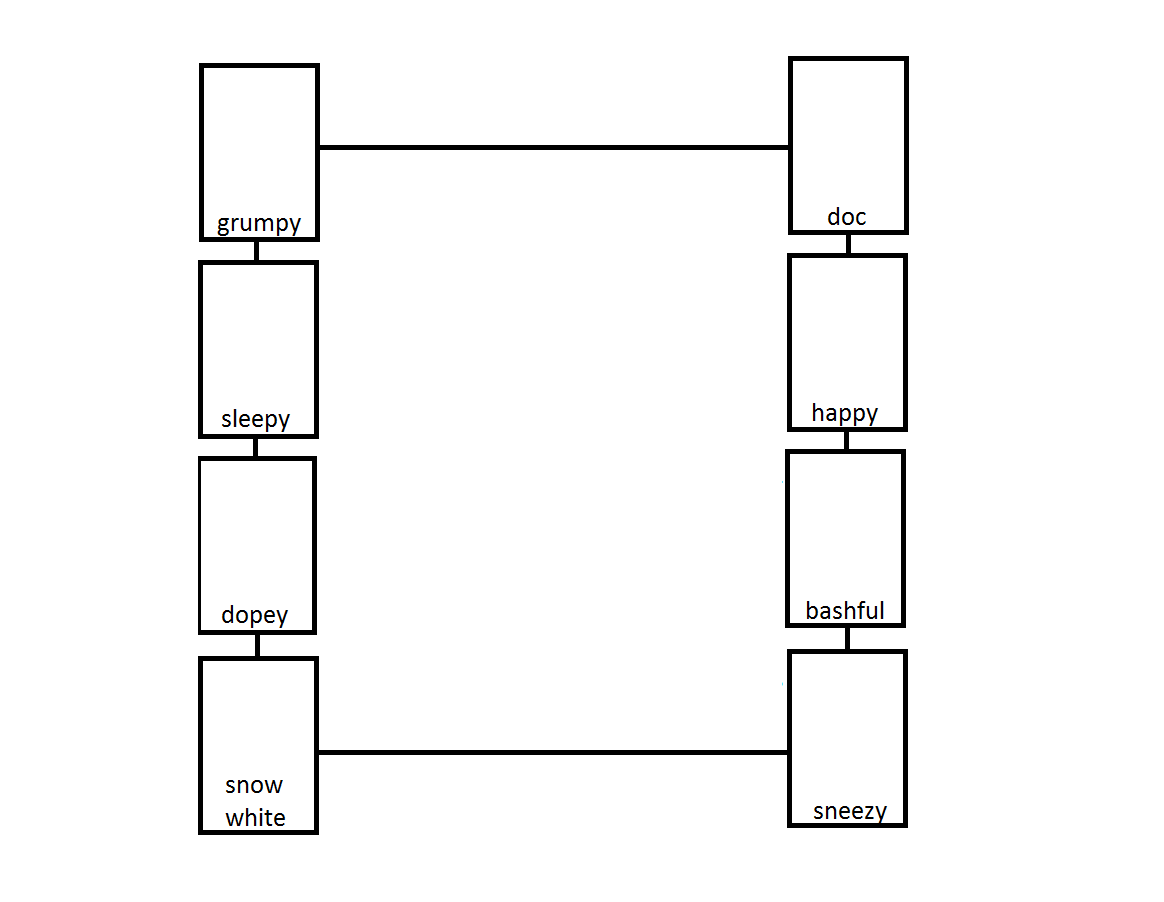
\includegraphics[width=0.75\textwidth]{ring.png}
	\label{fig:ring}
\end{figure}

\begin{figure}[tbh]
	\caption{Hypercube topology.}
	\centering
		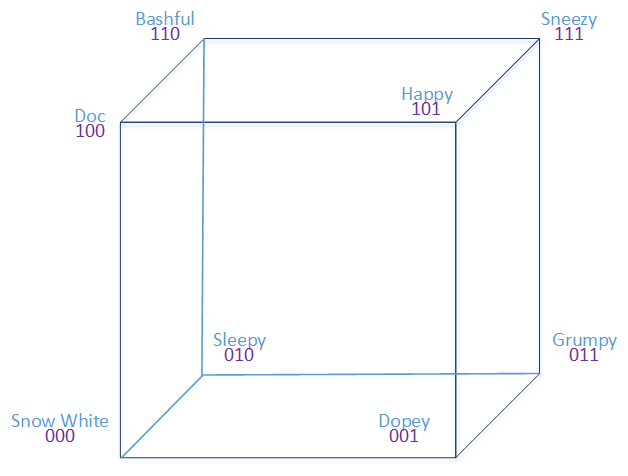
\includegraphics[width=0.75\textwidth]{HyperCube2.png}
	\label{fig:cube}
\end{figure}

\subsection{Changes to the Backlog}

Our final backlog changed over the course of the project. In the end, our goals going forward are as follows:

\begin{itemize}
	\item Benchmark the cluster using all availible cores.
	\item Benchmark different topologies not using a switch.
	\item Use the cluster to solve real-world problems.
	\item Continue looking at different possible communication methods with GPIO.
\end{itemize}



  %% All tracks
% New Templete!!
% !TEX root = DesignDocument.tex


\chapter{Prototypes}

% This chapter is for recording each prototype developed.  It is a historical record of what you accomplished in 464/465.   This should be organized according to Sprints.  It should have the basic description of the sprint deliverable and what was accomplished.  Screen shots, photos, captures from video, etc should be used.  

This is the overview of each prototype developed over the course of the project, organized by Sprints.

\section{Sprint 1 Prototype}

The work completed in the first sprint was largely information gathering. The goal was to determine which single-board computer best matched our needs for the cluster. We accomplished this by measuring the speed of each device in terms of addition, multiplication, division and the sine function accross numberous floating point values. 

\subsection{Deliverable}

\begin{itemize}
\item Mission Statement
\item User Stories
\item Number Generating Code
\item Benchmark Code
\item Benchmark Log
\item Signed Software Contract
\item Updated Design Document
\end{itemize}

\subsection{Backlog}

\begin{itemize}
\item Decide on a computer based on the results of the benchmarking
\item Calculate prices on supplies and computers while maintaining below the budget
\item Ordering said supplies and computers
\item Build the cluster to perform floating-point operations
\item Benchmark the cluster
\item Experiment with different topologies
\item Create a new mode of communication
\end{itemize}

\subsection{Success/Fail}

We successfuly found data for which device was faster, the cost of each device, and the power consumption while running. The benchmark results are in the following tables:

\begin{figure}[tbh]
	\caption{Performance of Raspberry Pi and ODROID}
	\centering
		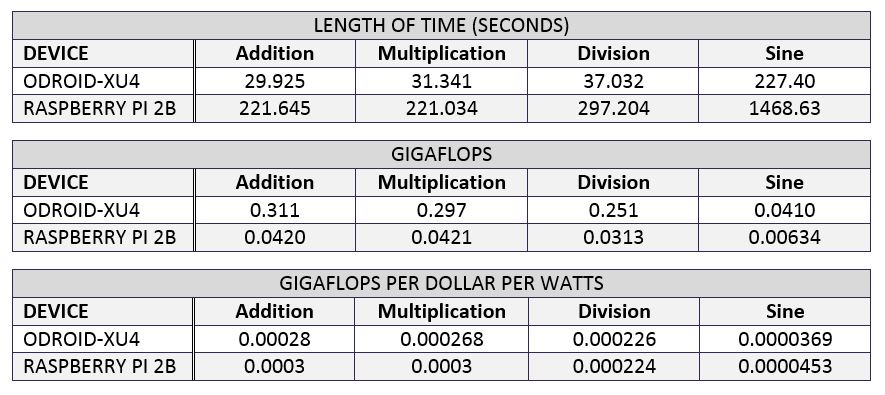
\includegraphics[width=0.75\textwidth]{pivsxu4table2.JPG}
\end{figure}

During the completion of this Sprint we encountered no significant failures. We were not set back from our schedule and were able to complete our Sprint goals.

\section{Sprint 2 Prototype}

This sprint also featured information gathering and preliminary work for knowlege we would need in creating the cluster. The decision was made to build the cluster out of ODroids, and the devices were ordered. The speed of the Ethernet port was tested while we waited for the devices to come in.

\subsection{Deliverable}

\begin{itemize}
\item Budget
\item Hardware Test
\item Switch Benchmark
\item Ethernet Benchmark
\item USB to Ethernet Benchmark
\item MPI Code
\item Message-Passing Protocol
\end{itemize}

\subsection{Backlog}

\begin{itemize}
\item Build the cluster
\item Code for the cluster
\item Benchmark the cluster
\item Experiment with different topologies
\item Create a new mode of communication
\end{itemize}

\subsection{Success/Fail} 

However, the ODroids were backordered, and took two weeks longer than expected to arrive. In the meantime, we were able to test the speed of the Ethernet port with the ODroid that we had, and we tested the speed of a USB to Ethernet device. We found that direct Ethernet connection using the built in ports was about 750 Mbps, and the USB to Ethernet devices gave 450 Mbps.

\section{Sprint 3 Prototype}

The Cluster of eight ODroid XU4s was assembled, completing our first physical prototype. The ODroids were attached to a piece of plexiglass, along with a power supply with a 5 volt power cord for each ODroid, and an 8 port switch. The end result is pictured in the following figure.

\begin{figure}[tbh]
	\caption{Cluster in Star Topology.}
	\centering
		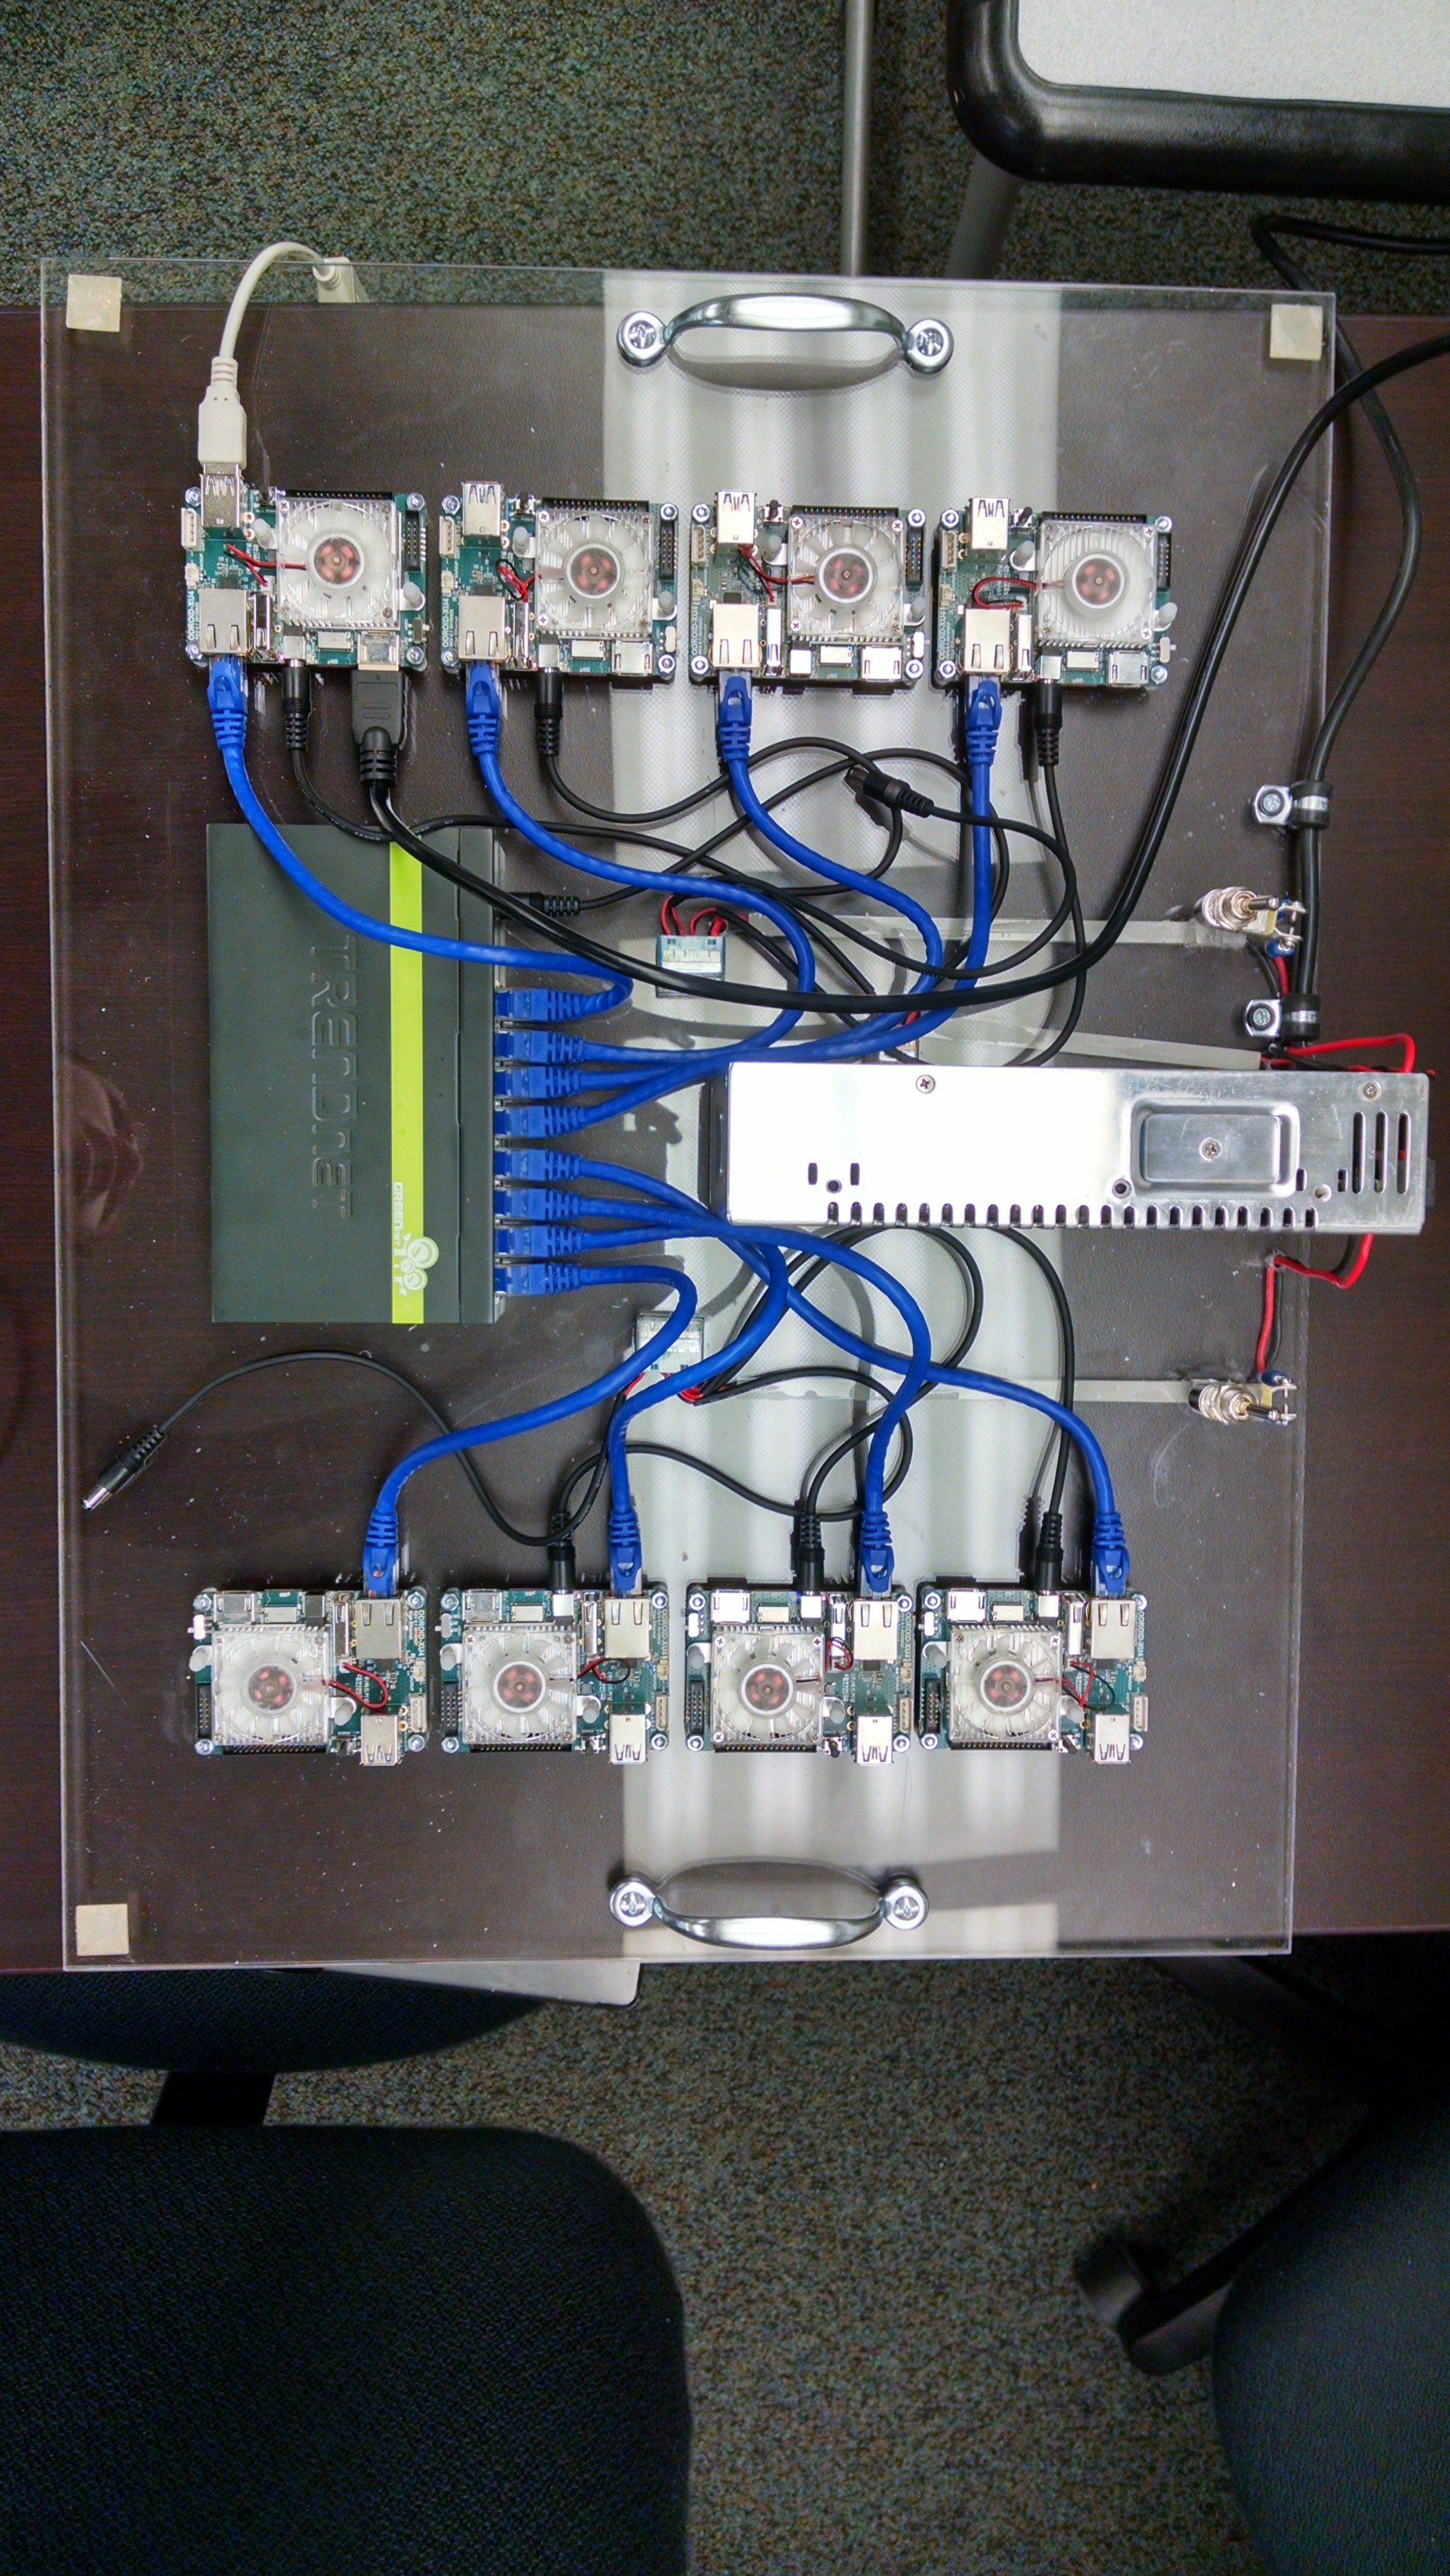
\includegraphics[width=0.75\textwidth]{IMG_20151201_104751350_HDR.jpg}
\end{figure}

On the software side, each ODroid was configured for our needs. First, each was assigned a static IP address in the network 192.168.0.X, and given it's hostname in accordinace with our naming convention of Snow White and the seven dwarfs. The final configuration for this sprint was to use RSA keys to allow each device to SSH to each other seven without prompting for a password. This was essential to allow MPI code to run. We also created some helper scripts to set up the cluster when it was booted. These included a script to use NFS to mount the /home directory of Snow White on the /home directory of the dwarfs. This was also essential to let MPI code located in the /home of Snow White to run on the cluster, as the same executable would be found in the same path on the dwarfs. We also created a script to shutdown the dwarfs from Snow White. 

\subsection{Deliverable}

\begin{itemize}
\item Built cluster
\item MPI code
\item Mounted home directory
\item Shutdown script
\item Mounting script
\item LINPACK and ATLAS installed on ODROIDs
\item MPI installed on ODROIDs
\item Hostnames
\item Fixed IP Addresses
\item SSH configuration
\end{itemize}

\subsection{Backlog}

\begin{itemize}
\item Research new connection methods
\item Benchmark the cluster
\item Experiment with different topologies
\item Create a new mode of communication
\item Design documentation
\item Research symposium
\begin{enumerate}
\item Complete abstract
\end{enumerate}
\item Design Fair
\end{itemize}

\subsection{Success/Fail}

We succeeded in creating and configured the cluster. Our largest failure was a setback from improperly changing the /etc/fstab file and causing the dwarfs to not boot. The goal was to make the devices mount the /home directory of Snow White on boot, but was ineffective. After a few days we were able to read the MMC card with a MMC to USB device and edit the fstab file manually using a different computer.

\section{Sprint 4 Prototype}

This sprint was largely the completion of benchmarking the cluster. We downloaned the source for High Performance Linpack, a tool used to test the speed of supercomputers. It worked with OpenMPI and ATLAS, a linear algebra package. We also had to build ATLAS for ARM. The benchmarking was a success and we found the speed of the cluster using all cores on all devices. Once that was complete, we began looking in to USB and GPIO communication.

\subsection{Deliverable}

\begin{itemize}
\item Graphs of total gigaflops performed depending on amount of devices used.
\item Debian package of LINPACK for ARM.
\item Found USB communication to not be feasible.
\item Able to send bits over GPIO between ODroid devices.
\item MICS abstract.
\end {itemize}

\subsection{Backlog}

\begin{itemize}
\item MICS presentation.
\item SDSMT Research Symnposium.
\item Design Documentation.
\item Design Fair.
\end{itemize}

\subsection{Success/Fail}

We successfully bencharked the cluster using Linpack. Results are shown in the following graph:

\begin{figure}[tbh]
	\caption{Linpack results.}
	\centering
		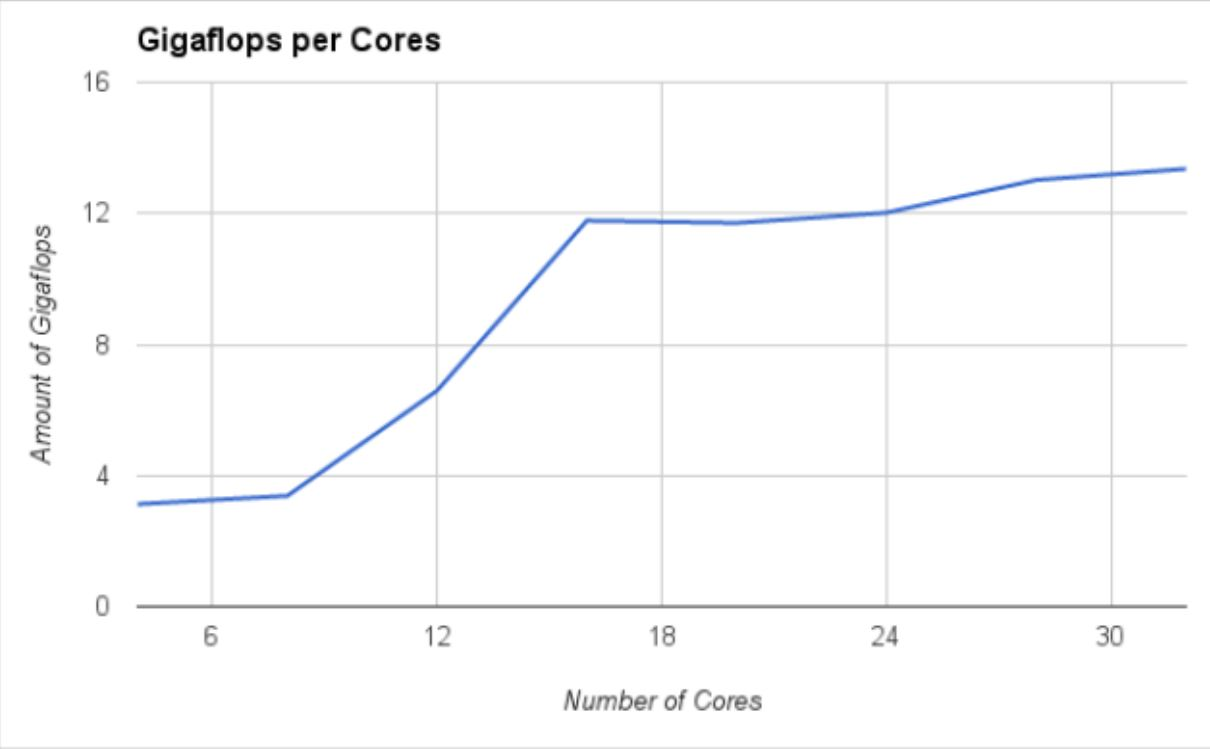
\includegraphics[width=0.75\textwidth]{minimalgraph.JPG}
\end{figure}

\section{Sprint 5 Prototype}

For this sprint, we tested the USB and GPIO communication. We were able to communicate over GPIO using the library WiringPi. In order to be able to do so, we had to install the source code on the ODROIDs and build it. We ran in to a few issues originally. First, the operatin system installed was not at it's most recent version, and therefore unable to work with the WiringPi libraries. We had to update each kernel individually, as shown in Figure~\ref{fig:purple} Once that was done, we still had to be able to use the library correctly. Extensive documentation existed for use with Raspberry Pis, but not for ODROID XU4s. Therefore, through a process of trial and error to see which WiringPi pin number corresponded to each physical pin, we were able to create our own in Figure~\ref{fig:gpio} 

\begin{figure}[tbh]
	\caption{Linpack results.}
	\centering
		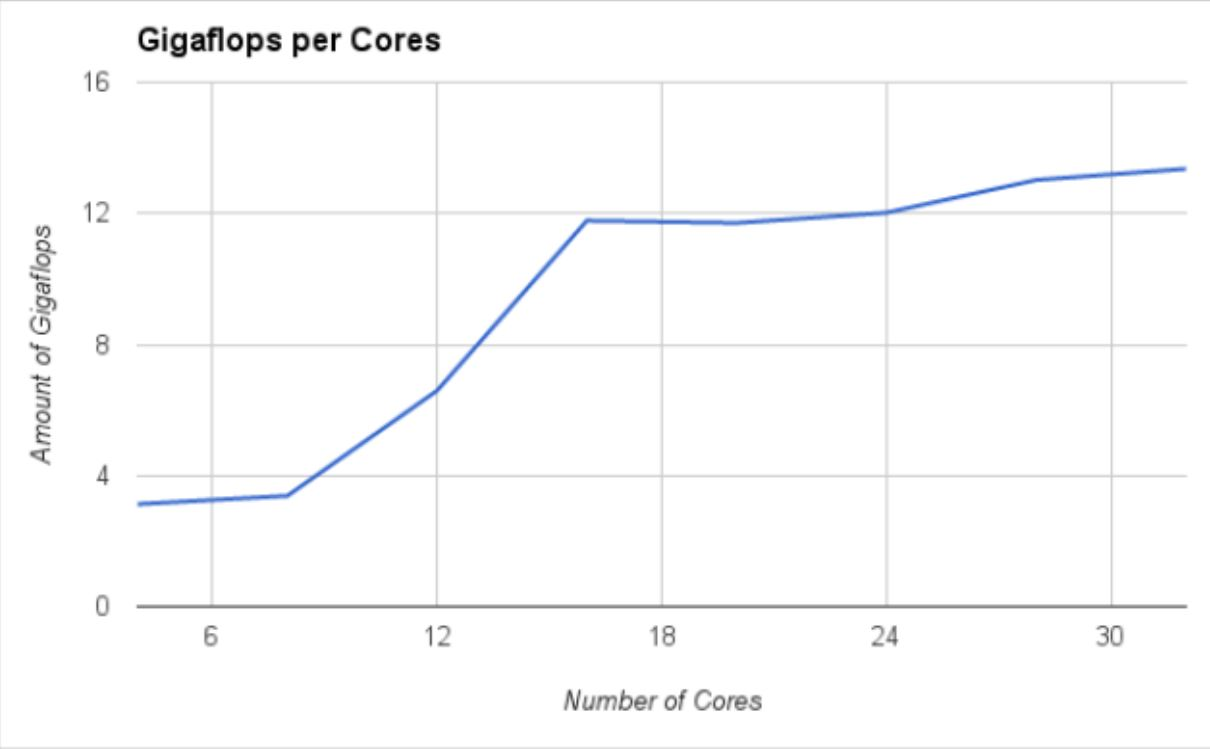
\includegraphics[width=0.75\textwidth]{minimalgraph.JPG}
	\label{fig:minimal}
\end{figure}

\begin{figure}[tbh]
	\caption{Updating kernel.}
	\centering
		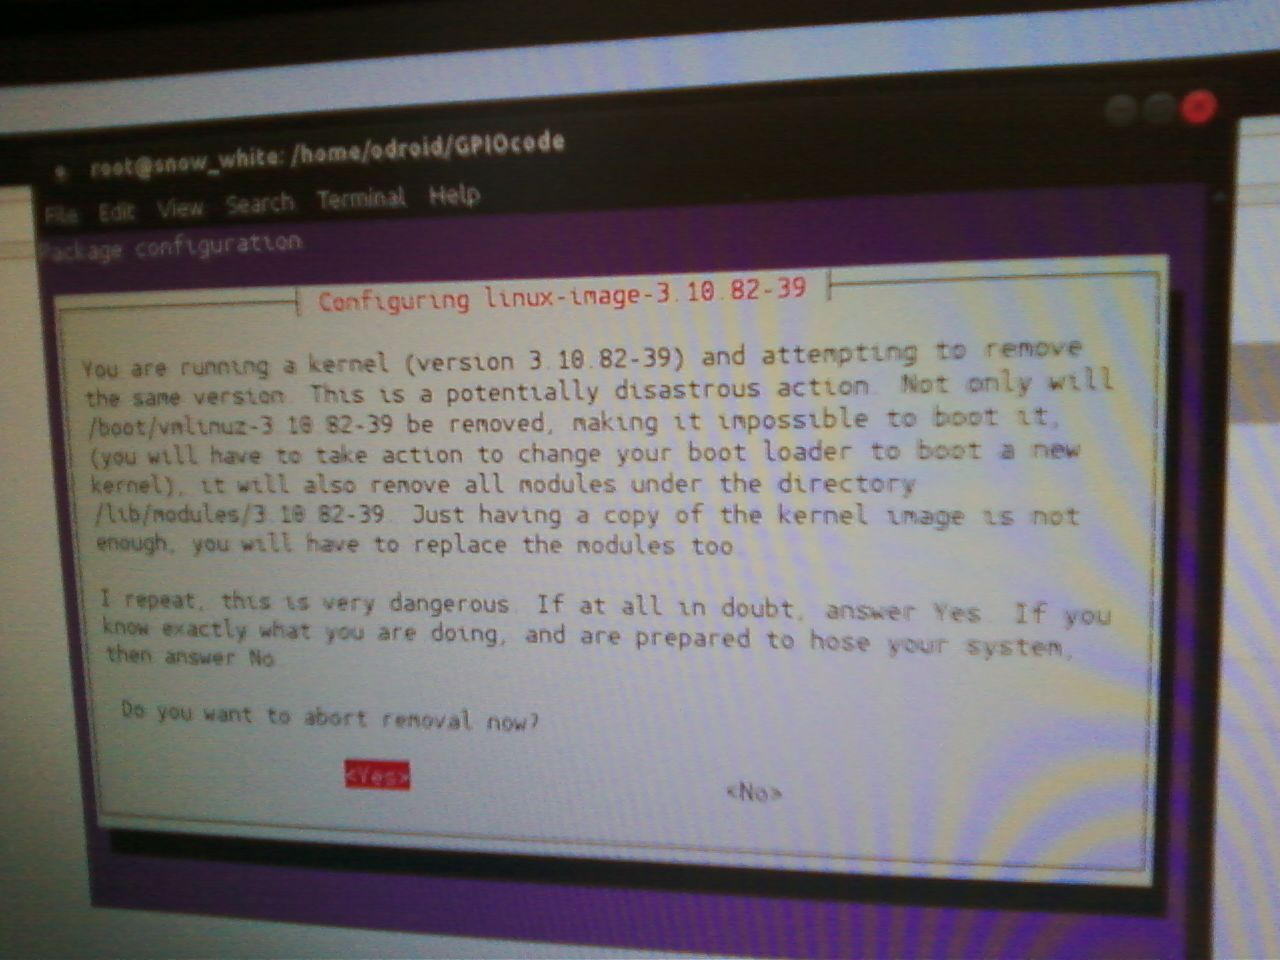
\includegraphics[width=0.75\textwidth]{PurpleScreen.jpg}
	\label{fig:purple}
\end{figure}

\begin{figure}[tbh]
	\caption{WiringPi values.}
	\centering
		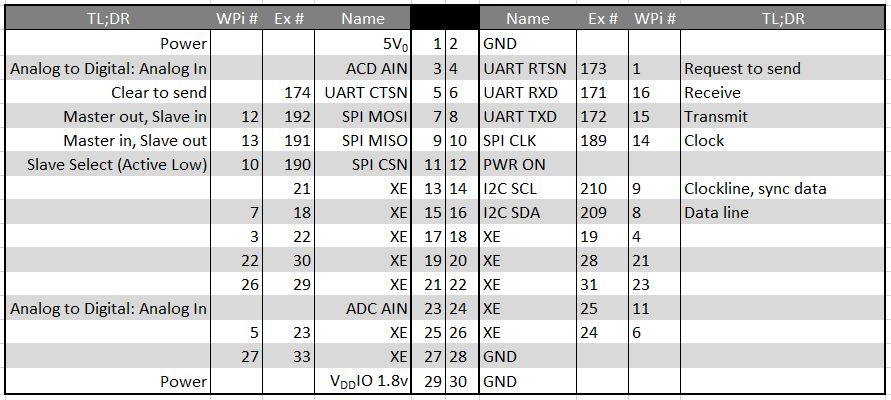
\includegraphics[width=0.75\textwidth]{gpio.JPG}
	\label{fig:gpio}
\end{figure}

It was determined that netiher were pratcical for our purposes due to the scope of the project and the low speed. In order to try and increase the gigaflops of the system, we instead experimented with different topologies. We used USB to Ethernet devices to add more network interfaces to each ODroid and attach them in a ring. This allowed a different method of communication instead of using the switch. In order for communication to work, we had to assign IP addresses to the new interfaces on the 192.168.X.Y network, where X is the ODroid number 0-7, and Y was the number of the interface for that device. We also created our abstract for the SDSMT Reseach Symposium, and for the MICS conference. We wrote a first draft of the MICS paper as well in preparation of our presentation in April 23rd. 

\subsection{Deliverable}

\begin{itemize}
\item Design for the hypercube and ring topology.
\item Routing tables for each of the ODROIDs.
\item The cluster connected with new topology.
\item Able to send bits over GPIO between ODroid devices.
\item Acceptance into MICS.
\item First draft of MICS paper.
\item SDSMT Research Symposium abstract.
\end{itemize}

\subsection{Backlog}

\begin{itemize}
\item MICS presentation.
\item SDSMT Research Symnposium.
\item Completed hypercube cluster.
\item Conglomerate data results.
\item Design Documentation.
\item Design Fair.
\end{itemize}

\subsection{Success/Fail}

Our largest failure this sprint was our inability to benchmark the different topologies. We found that MPI does not work with different network interfaces on the same subnet. Even after changing the IP addresses so that each IP address was on a different subnet, the code still did not work. Therefore, we are unable to use Linpack to benchmark the cluster in the ring or hypercube topology.
  %% All tracks %%NEW!!!!!!!!!!!!
% New Templete!
% !TEX encoding = UTF-8 Unicode
% !TEX root = DesignDocument.tex

%% This is not generally for the research track

\chapter{Release -- Setup -- Deployment}
%%This section should contain any specific subsection regarding specifics in releasing, setup, and/or deployment of the system. 

\section{Deployment Information and Dependencies}
%%Are there dependencies that are not embedded into the system install? 

\section{Setup Information}
%%How is a setup/install built? 

\section{System  Versioning Information}
%%How is the system versioned? 
  %% Normally not research track
% !TEX root = SystemTemplate.tex

\chapter{User Documentation}

This section should contain the basis for any end user documentation for the system. 
 End user documentation would cover the basic steps for setup and use of the system. 
 It is likely that the majority of this section would be present in its own document 
to be delivered to the end user.  However, it is recommended the original is contained 
and maintained in this document. 

%\newpage   %% 
%%  The user guide can be an external document which is included here if necessary ...
%%  a single source is the way to go.

\section{User Guide}

The source for the user guide can go here.    You have some options for how to handle the user docs.  If you have some {\tt newpage} commands around the guide then you can just print out those pages.   If a different formatting is required, then have the source in a separate file {\tt userguide.tex} and include that file here.  That file can also be included into a driver (like the senior design template) which has the client specified formatting.  Again, this is a single source approach.   


%% \newpage  %%  if needed ...
\section{Installation Guide}


%% \newpage  %%  if needed ...
\section{Programmer Manual}

 %% All tracks
%% New templete!!
% !TEX root = DesignDocument.tex


%%\chapter{Class Index}
%%%old
\section{Class List}
Here are the classes, structs, unions and interfaces with brief descriptions\-:\begin{DoxyCompactList}
\item\contentsline{section}{\hyperlink{class_poly}{Poly} }{\pageref{class_poly}}{}
\end{DoxyCompactList}

%%\chapter{Class Documentation}
%%\hypertarget{class_poly}{\section{Poly Class Reference}
\label{class_poly}\index{Poly@{Poly}}
}
\subsection*{Public Member Functions}
\begin{DoxyCompactItemize}
\item 
\hyperlink{class_poly_aa3def076b74bed67904976ad4f9fe9b1}{Poly} ()
\item 
\hyperlink{class_poly_a2f8530284140c31c0aa391dd4d0b61be}{$\sim$\-Poly} ()
\item 
int \hyperlink{class_poly_a14a7ad77ce612b0c54f531d307ee4b39}{myfunction} (int)
\end{DoxyCompactItemize}


\subsection{Constructor \& Destructor Documentation}
\hypertarget{class_poly_aa3def076b74bed67904976ad4f9fe9b1}{\index{Poly@{Poly}!Poly@{Poly}}
\index{Poly@{Poly}!Poly@{Poly}}
\subsubsection[{Poly}]{\setlength{\rightskip}{0pt plus 5cm}Poly\-::\-Poly (
\begin{DoxyParamCaption}
{}
\end{DoxyParamCaption}
)}}\label{class_poly_aa3def076b74bed67904976ad4f9fe9b1}
My constructor \hypertarget{class_poly_a2f8530284140c31c0aa391dd4d0b61be}{\index{Poly@{Poly}!$\sim$\-Poly@{$\sim$\-Poly}}
\index{$\sim$\-Poly@{$\sim$\-Poly}!Poly@{Poly}}
\subsubsection[{$\sim$\-Poly}]{\setlength{\rightskip}{0pt plus 5cm}Poly\-::$\sim$\-Poly (
\begin{DoxyParamCaption}
{}
\end{DoxyParamCaption}
)}}\label{class_poly_a2f8530284140c31c0aa391dd4d0b61be}
My destructor 

\subsection{Member Function Documentation}
\hypertarget{class_poly_a14a7ad77ce612b0c54f531d307ee4b39}{\index{Poly@{Poly}!myfunction@{myfunction}}
\index{myfunction@{myfunction}!Poly@{Poly}}
\subsubsection[{myfunction}]{\setlength{\rightskip}{0pt plus 5cm}int Poly\-::myfunction (
\begin{DoxyParamCaption}
\item[{int}]{a}
\end{DoxyParamCaption}
)}}\label{class_poly_a14a7ad77ce612b0c54f531d307ee4b39}
my own example function fancy new function

new variable 

The documentation for this class was generated from the following file\-:\begin{DoxyCompactItemize}
\item 
hello.\-cpp\end{DoxyCompactItemize}

  %% All tracks
% !TEX encoding = UTF-8 Unicode
% !TEX root = DesignDocument.tex

\chapter{Business Plan}



\section{Business Model}

\section{Market and Competition}

\section{Regulatory environment}

\section{Intellectual Property and Freedom to Operate}

\section{Management Team and Advisors}

\section{Sources and Uses of Capital}

\section{Financial Statements}

\section{Metrics and Milestones}

\section{Exit Plan}

   %% Entrepreneur track only 
% New Templete!!
% !TEX root = DesignDocument.tex


\chapter{Experimental Log}

For research projects one needs to keep a log of all research/lab activities.   

%% If you have multiple labs, you may want to break the labs into sections, check 
%% with the profession on format.
%% \section{Lab 1}

%%\begin{description}
%%\item [10/15/15]  Ran modified filter on data sets 1 - 6.  Results were ...
%%\item [10/17/15]  Changed tolerance on sensor and collected data.  These ...
%%\end{description}

\section{Benchmarking the Individual Computers}

\begin{description}
\item [9/17/15]  PcDuino isn't working according to Dr. Karlsson. The PcDuinos are about \$160 each, so chances were that the PcDuino wasn't going to be selected for the cluster. We will not put the PcDuino in consideration with our benchmarking. \\

\item [9/17/15]  PcDuino isn't working according to Dr. Karlsson. The PcDuinos are about \$160 each, so chances were that the PcDuino wasn't going to be selected for the cluster. We will not put the PcDuino in consideration with our benchmarking. \\

\item [9/22/15] We begin work on benchmarking the remaining candidates. The code we will be using to benchmark the two devices will test the addition, multiplication, division, trigonmetric function in single and double point precision of two massively large arrays filled with random numbers. \\

\item [9/29/15] OpenMP is added to the benchmark code so the program runs on all cores. Results are as follows: \\

\begin{center}
\begin{tabular}{ | l || l | l | l | l | }
\hline
\multicolumn{5}
{ |c| }{ Length of Time (seconds) } \\
\hline
Device & Addition & Multiplication & Division & Sine \\
\hline
ODroid 4xU & 29.925 & 31.341 & 37.032 & 227.40 \\
\hline
Raspberry Pi 2B & 221.645 & 221.034 & 297.204 & 1468.63 \\
\hline
\end{tabular}
\end{center}

\item [9/30/15] The gigaflops are calculated. \\
\begin{center}
\begin{tabular}{ | l || l | l | l | l | }
\hline
\multicolumn{5}
{ |c| }{ Gigaflops } \\
\hline
Device & Addition & Multiplication & Division & Sine \\
\hline
ODroid 4xU & 0.311 & 0.297 & 0.251 & 0.0410 \\
\hline
Raspberry Pi 2B & 0.0420 & 0.0421 & 0.0313 & 0.00634 \\
\hline
\end{tabular}
\end{center}

\item [10/1/15] The wattage is measured when the devices are running these operations. Using the wattage, the metric of GFlops/Dollar/Watt is calculated. \\

\begin{center}
\begin{tabular}{ | l || l | l | l | l | }
\hline
\multicolumn{5}
{ |c| }{ Gigaflops per Dollar per Watts } \\
\hline
Device & Addition & Multiplication & Division & Sine \\
\hline
ODroid 4xU & 0.00028 & 0.000268 & 0.000226 & 0.0000369 \\
\hline
Raspberry Pi 2B & 0.0003 & 0.0003 & 0.000224 & 0.0000453 \\
\hline
\end{tabular}
\end{center}

\item [10/1/15] The results show that the Raspberry Pi and the ODroid perform nearly the same. The Raspberry Pi in our benchmarking proved the best. However, it is inconclusive as to which computer will be used. \\

\item [10/24/15] Decided to go with the ODroid. Performance and the number of ports outweighted the cost of the Raspberry Pi. \\

\end{description}

\section{Ethernet Benchmark}
\begin{description}
\item [10/25/15] Created network between a machine with gigabit Ethernet port and ODROID. Installed iperf, a tool in the standard Debian repositories to text the network speed, on both the server machine and ODROID. \\

This text can be run over the existing network by the following steps: \\
%add dollar signs or >
ssh andrewdesktop@108.107.223.45 \\
Password: design \\
iperf -s \& \\
Leave that running in the background. \\
ssh odroid@10.42.0.2 \\
Password: odroid \\
iperf -c 10.42.0.1 \\
This will take a few seconds to run then give the network speed. The network 10.42.0.1 is over a 1000 Mbps wired connection between the ODROID and andrewdesktop. \\

\begin{center}
\begin{tabular}{ | l || l | }
\hline
\multicolumn{2}
{ |c| }{ Ethernet Speed } \\
\hline
Device & Speed (Mbps) \\
\hline
ODroid XU4 & 615 - 625 \\
\hline
\end{tabular}
\end{center}

\end{description}

\section{Hardware Test}
\begin{description}
\item [11/03/15] All eight ODroids are functional. To test them, each device was connected to a router with internet access via Ethernet. A monitor was connected through HDMI, and the mouse and keyboard were connected to both USB 3.0 ports to ensure they worked. The packages mpi-default-dev and openmpi-bin were installed. The test MPI code found this directory and successfully compiled and executed. No issues found on any device. \\
\end{description}

\section{Switch Benchmark}
\begin{description}
\item [11/03/15] With two ODROID devices attached to the switch via direct ethernet (no USB 3.0 to ethernet adapter), the connection speed was tested. This was accomplished by one device running: \\

%add $ or >
iperf -s \\

and the other running: \\

%use <>
iperf -c [IP of the first device]

\begin{center}
\begin{tabular}{ | l || l | }
\hline
\multicolumn{2}
{ |c| }{ Switch Speed } \\
\hline
Device & Speed (Mbps) \\
\hline
ODroid XU4 & 775 - 800 \\
\hline
\end{tabular}
\end{center}

This is notably faster than the previous benchmark between one ODROID and a non-ODROID machine not using a switch.
\end{description}

\section{USB to Ethernet Benchmark}
\begin{description}
\item [11/03/15] Tested speed of USB 3.0 to ethernet adapter using iperf. Found slower than direct ethernet conection. Test speeds varied greatly, between 300 Mbps and 700 Mbps. The USB ethernet adapted was faster acting as a server than a client with the highest value as a client being only about 475 Mbps. In contrast, the ethernet connections were consistent reguarless of which device was the client or server, and stayed between 775 and 800 Mbps. 

\begin{center}
\begin{tabular}{ | l || l | }
\hline
\multicolumn{2}
{ |c| }{ USB 3.0 to Ethernet Adapter Speed } \\
\hline
Device & Speed (Mbps) \\
\hline
ODroid XU4 & 300 - 700 \\
\hline
\end{tabular}
\end{center}

Additionally, there hasn't been a found way to connect two devices over USB-ethernet to ethernet directly. When attached to the switch, the devices can communicate; however, if we were using the USB to ethernet adapters, they would be directly connected, without the switch. Therefore, being unable to direct connect devices defeats the purpose of the adapters. In conclusion, the drastically lower speed of the USB to Ethernet adapters and the inability to directly connect devices means that the devices are very unlikely to useful for our purposes. \\

\item [11/05/15] There isn't a found way to connect two devices over USB-ethernet to ethernet directly. When attached to the switch, the devices can communicate. If using the USB to ethernet adapter, they would be directly connected without the switch. Therefore, it was unable to directly connect devices. \\ \\
The drastically lower speed of the USB to ethernet adapters and the inability to directly connect the devices means that the devices are very unlikely to be useful for this project.
\end{description}

%Sprint 3


% Sprint 4
\section{Auto-Mounting Snow White's Home Directory}
\begin{description}
\item [1/16/16] Attempting to auto-mount Snow White's homedirectory onto the dwarfs. Changed Sleepy's fstab file with this line: \\ \\
%need to figure out > in front of the line below
192.168.1.11:/home /hom nfs auto 0 0 \\ \\
We can now mount Snow White's home directory automatically onto Sleepy. Adding this to other dwarfs' fstab file.
\end{description}

\section{Creating a Debian Package}
\begin{description}
\item [1/18/16] To create a simple Debian package, we followed the instructions located at:\\ \\
\url{https://wiki.debian.org/IntroDebianPackaging}\\ \\
%add the steps here?
This let us create a Debian package. Going forward, the next step is to use the instructions to make HPLinpack into a Debian package.
\end{description}

\section{USB to USB Communication}
\begin{description}
\item [1/26/16] Figuring out how to communicate through USB. In /etc/network/interface, changed USB's from static to dhcp. Then performed sudo ifup usb0.
Setting up the USB IP Addresses:
Go the the ODROID to change.


% 	\$ wget http://tex.stackexchange.com
	%\$ sudo modprob g_ether
	%\$ dmesg
	%\$ sudo ifconfig usb0 ipaddress 
	%\$ config

%\langle dog \rangle

Verify the USB IP address was changed.

Changed Doc, Happy, Bashful, and Sneezy's USB IP addresses:
	\begin{itemize}
		\item Doc - 192.168.1.25
		\item Happy - 192.168.1.26
		\item Bashful - 192.168.1.27
		\item Sneezy - 192.168.1.28
	\end{itemize}
\item[2/1/16] Over USB 2.0, it is possible to use USB crossover cables to simulate Ethernet over USB. The same technology is possible for USB 3.0, but no operating system currently supports it, Linux or otherwise. As such, direct communication would have to be done in a different way than Ethernet, such as PyUSB. However, there is no found way to communicate from hsot node to another host node using PyUSB.
\end{description}

\section{GPIO Communication}
\begin{description}
\item [2/4/16]  Connected index pin 8 (UART TXD) (Export Pin 172) on Doc to index pin 6 (UART RXD) (Export Pin 171) on Happy. Communicating by changing the physical bit in the corresponding GPIO export pin file (not the physical index number).  \\
%put a gpio diagram somewhere and reference it here

In Happy: \\
%add > before these
cd /sys/class/gpio\\
Mount the export pin: \\
echo 171 greatherthan export\\
It makes gpio171\\
cd gpio171 \\
Edit the text file direction:\\
echo in greaterthan direction \\

In Doc: \\
%add the > before these
cd /sys/class/gpio \\
echo 172 greaterthan export \\
It makes a directory for that pin number. \\
cd gpio172 \\
Edit the text file direction to out: \\
echo out greaterthan direction \\
Edit the text file direction: \\
echo 1 greatherthan value\\

In Happy: \\
cd /sys/class/gpio/gpio171 \\
echo value \\
It'll print 1\\

Repeat with value 0. Happy's value will be 0. \\

To unmount the GPIO Export Pin: \\
In Happy: \\
cd /sys/class/gpio \\
echo 171 greaterthan unexport \\

In Doc: \\
cd /sys/class/gpio \\
echo 172 greaterthan unexport

\item [2/11/16] Successfully got wiringPi to work between two dwarfs. We got 0.61 MBits/sec on GPIO with one pin. Communication speed between two dwarfs through Ethernet was 750 MBits/sec. This was found using iperf. GPIO was 120 times slower than Ethernet. It was concluded that GPIO will not be continued for this project.

\end{description}

\section{Updating Kernel}
\begin{description}
\item [2/6/16] Trying to install the wiringPi2 library on the ODROIDs to communicate via GPIO. Our online sources said we need to update the kernels. \\

Change the fstab so it doesn't mount Snow White's home directory automatically. (Comment out) \\
Edit etc/interfaces, comment out so the ODROID can connect to the internet.\\
Reboot the ODROID.\\
Connect to internet ethernet while rebooting. \\
Check the current kernel: \\
uname -a \\
Update the repos: \\
sudo apt-get update \\
Upgrade the kernel: \\
apt-get upgrade linux-image-xu3 \\
Got a purple screen prompting if we want to continue and if we know what we're doing. Continued. \\
Ignore warning errors. \\
Check the current kernel to see if it successfully updated: \\
uname -a \\
Upgrade all of the packages for the kernel: \\
sudo apt-get update \&\& sudo apt-get dist upgrade
\end{description}   %% Research track  only
% !TEX root = DesignDocument.tex


\chapter{Research Results}

%%This chapter describes the results and conclusions of your research.   This would be the final report for a research project.  

By the conclusion of the project, many different results had been drawn about several aspects of the cluster. The first are the results of testing of each single device. Then, the maximum amount of Gigaflops the cluster can produce with LINPACK was found. GPIO and USB communication were also analyzed. 

\section{Result 1}

First, the Raspberry PI 2B and ODROID XU4 were tested individually to find which was faster. The results are shown in Figure~\ref{pivodroid} along with the final metric of Gigaflops per dollar per watt. It was found that the Raspberry Pi cost \$35 and used 4 watts of power while running, and the ODroid cost \$75 and used 15 watts. 

\begin{figure}[tbh]
\begin{center}
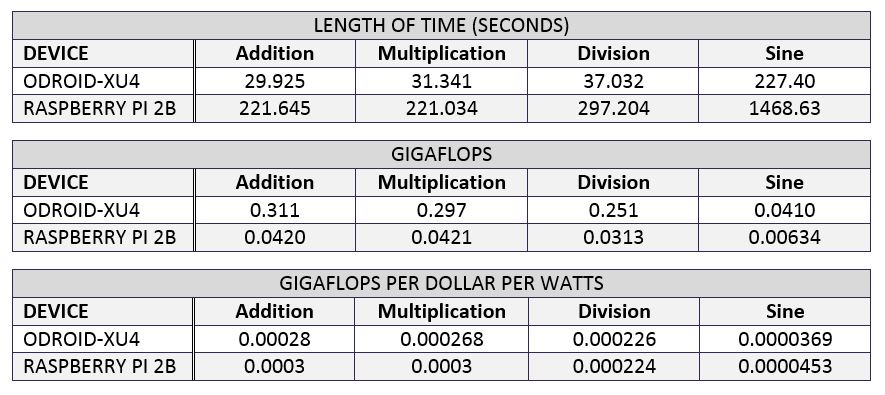
\includegraphics[width=0.75\textwidth]{pivsxu4table2.JPG}
\end{center}
\caption{PI vs ODROID results. \label{pivodroid}}
\end{figure}

\section{Result 2}

We also measured the speed of the Ethernet connections using the tool iperf. It was testing by directly connecting two devices Ethernet to Ethernet, and connected over the switch. Also, using USB to Etherent devices to create new network interfaces on the ODroids was tested by connecting those ports to the built in Ethernet ports. The results are shown in Table~\ref{ethernet}

\begin{table}[tbh]
\caption{Ethernet speeds. \label{ethernet}}
\begin{center}
\begin{tabular}{|r|l|}
  \hline
  Ethernet to Ethernet & 750 Mbps \\
  USB to Ethernet &  450 Mbps \\ 
  Ethernet over switch & 750 Mbps \\
  \hline
\end{tabular}
\end{center}
\end{table}

\section{Result 3}

Direct USB to USB communication was also tested. The devices were attached by USB 3.0 ports with the intent to use them to pass information between. However, further research proved that there is no current way to transfer information from two hosts using USB 3.0. It can be done with USB 2.0 using crossover cables, but there does not exist any common operating system that supports the same feature with 3.0. Therefore, we did not benchmark USB 3.0 communication.

\section{Result 4}

Another alternate form of communication tested was GPIO. The library WiringPi was installed and used with C to read and write values to pins. It was found that communication was successful, but in order to make a protocol faster than Ethernet, even if we used all 40 pins to tranfer data, we would need each pin to send over 19.5 million bits per second, as per \begin{equation}(750 * 1024^{2}) / 40 \end{equation}WiringPi, in our preliminary testing, was only able to send about 500,000 bits per second on a pin. Therefore, it was concluded that our cluster would always be faster using Ethernet.

\section{Result 5}

Our final result was using LINPACK to test the amount of Gigaflops produced by the cluster. 

\begin{figure}[tbh]
\begin{center}
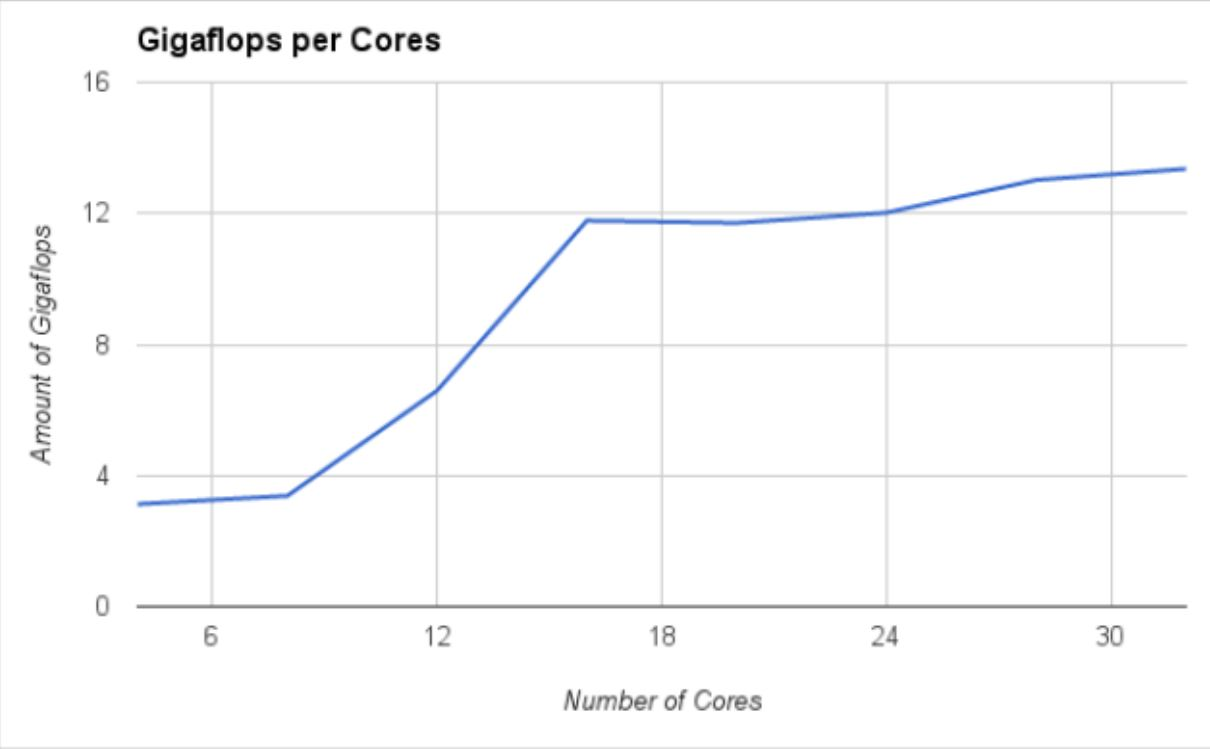
\includegraphics[width=0.75\textwidth]{minimalgraph.JPG}
\end{center}
\caption{LINPACK results. \label{linpackresults}}
\end{figure}

\section{Conclusions}

\section{Further work}  
  %% Research track  only

%%\bibliographystyle{plain}
%%\bibliography{designrefs.bib}
%%\addcontentsline{toc}{chapter}{Bibliography}


% We want to add the Software agreement to the end and number the
% pages separately from the document.  We don't want to do a standard
% chapter heading, but we do want it to appear in the table of contents
% and in the index used for on-line viewing.  We defined the \agreement
% macro to set things up for us.
\agreement

\chapter{Software Agreement}
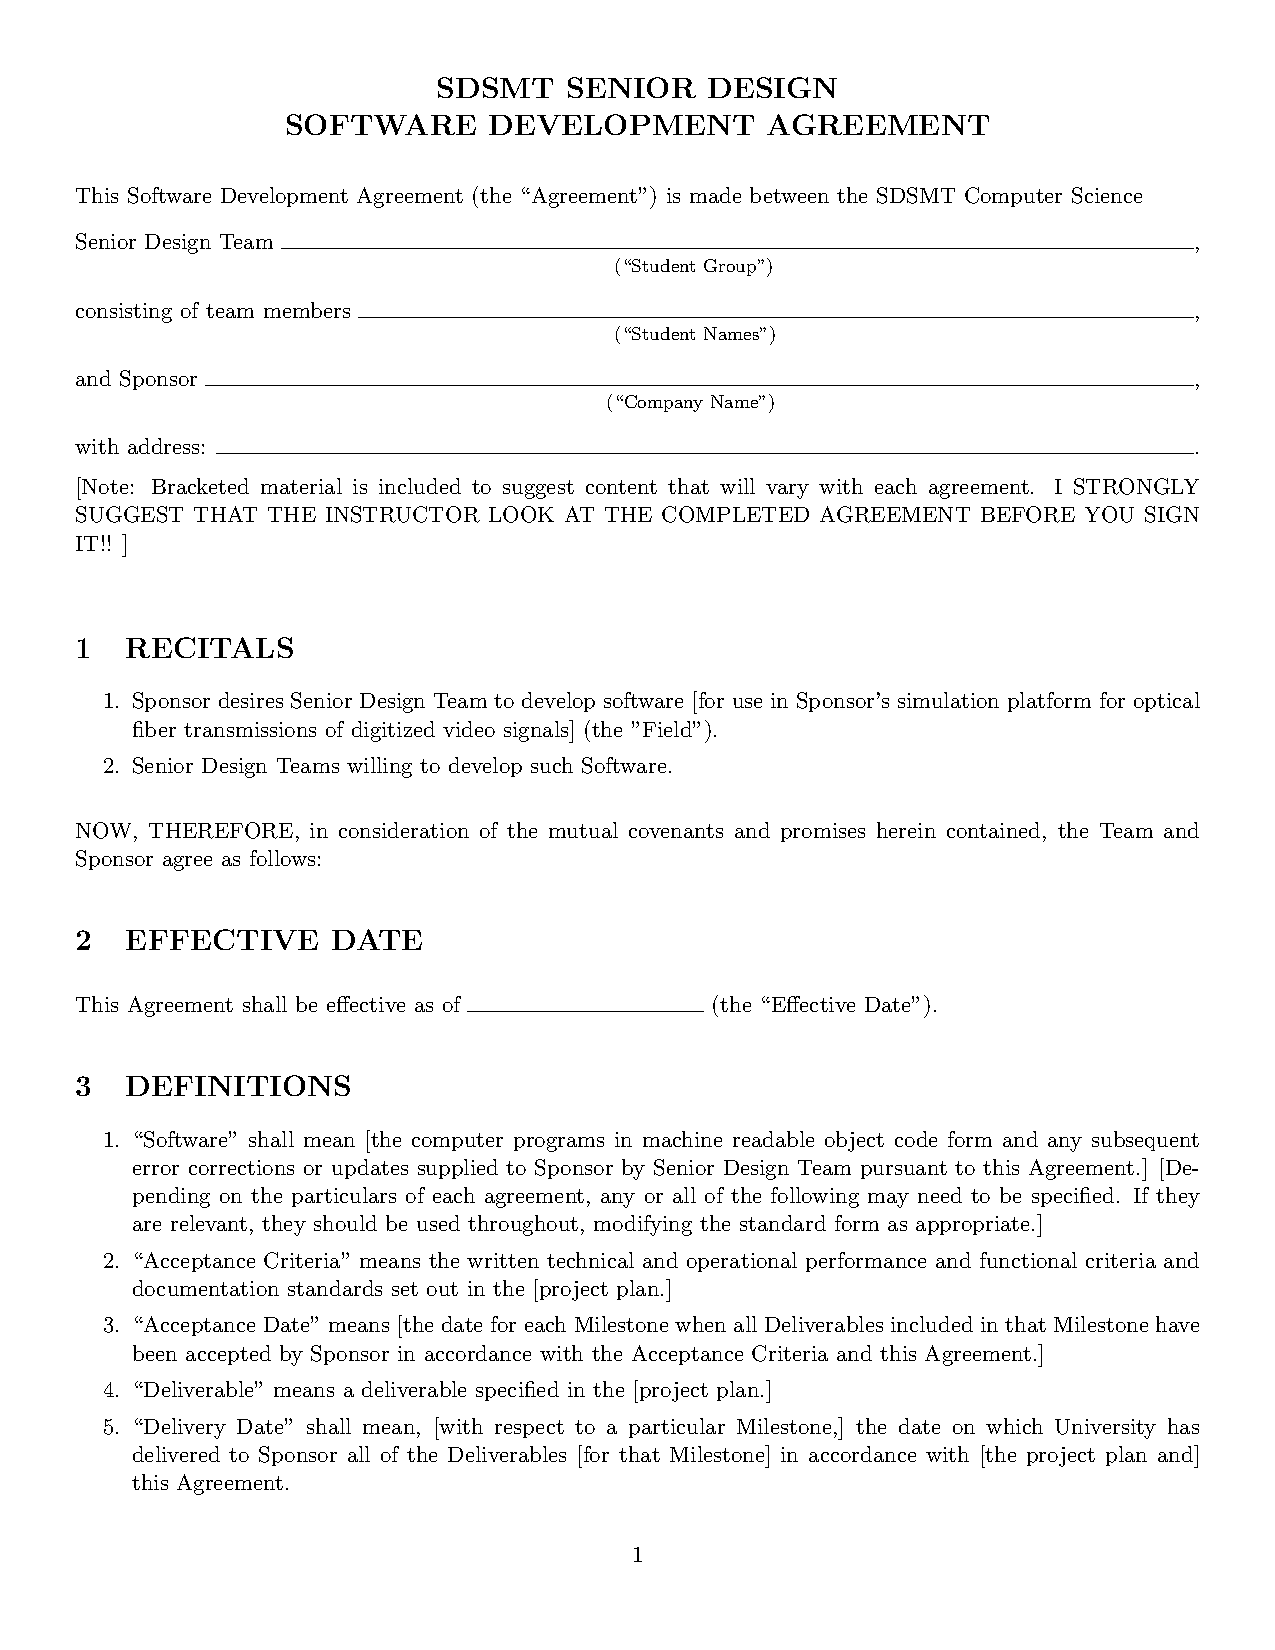
\includepdf[pages={1-5}]{SoftwareContract.pdf}

% In our style file, appendices are numbered with capital letters
\appendix

\chapter{Product Description}
%old

Write a description of the product to be developed.
Use sectioning commands as neccessary.
\vspace{2\baselineskip}

\centerline{\Large {\bf NOTE:} {\em This is part of the contract.}}



\chapter{Publications}   %% Research track 
% New Templete!!
% !TEX root = DesignDocument.tex


%%Research Track:  
%%This chapter will include any publications generated from the research.  Most likely these will be preprints and one will just include the pdf.

%\includepdf[pages={1-5}]{Pub1.pdf}
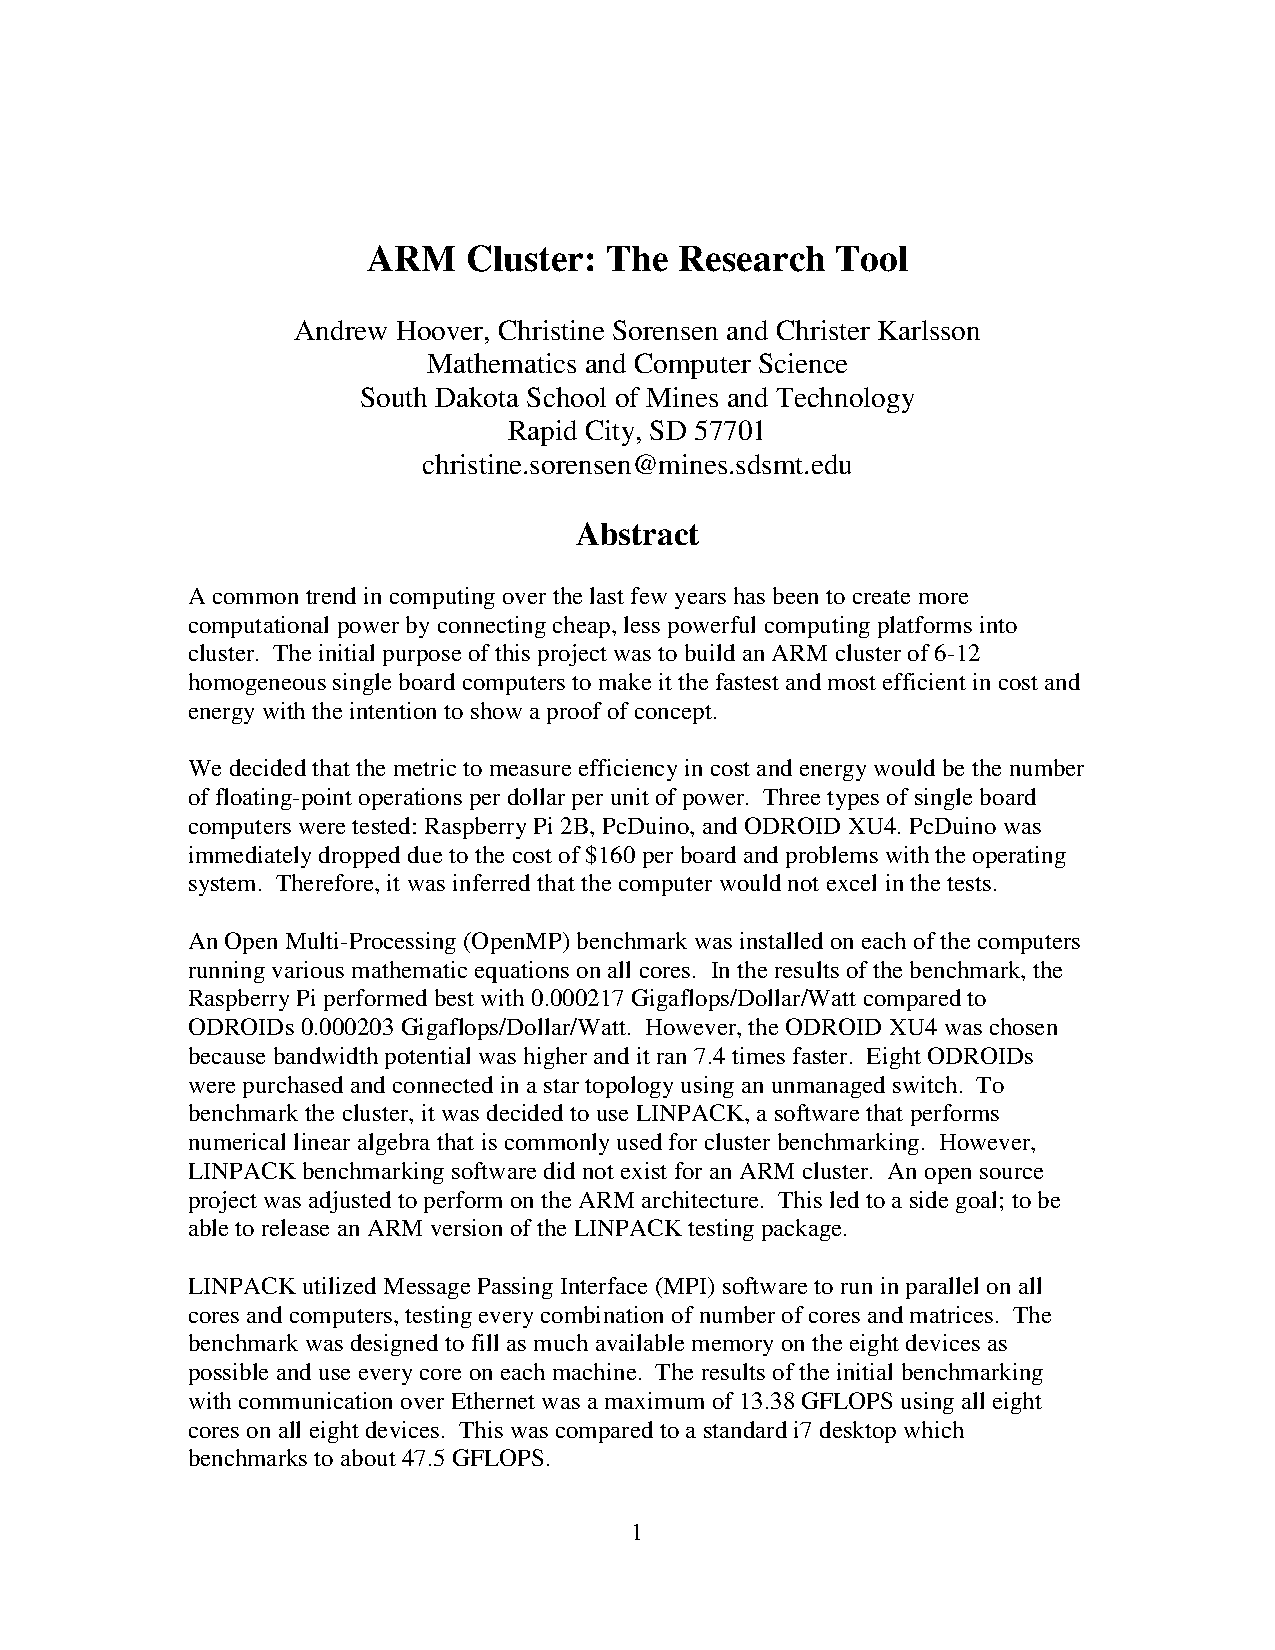
\includepdf[pages={1-2}]{MICSAbstract.pdf}
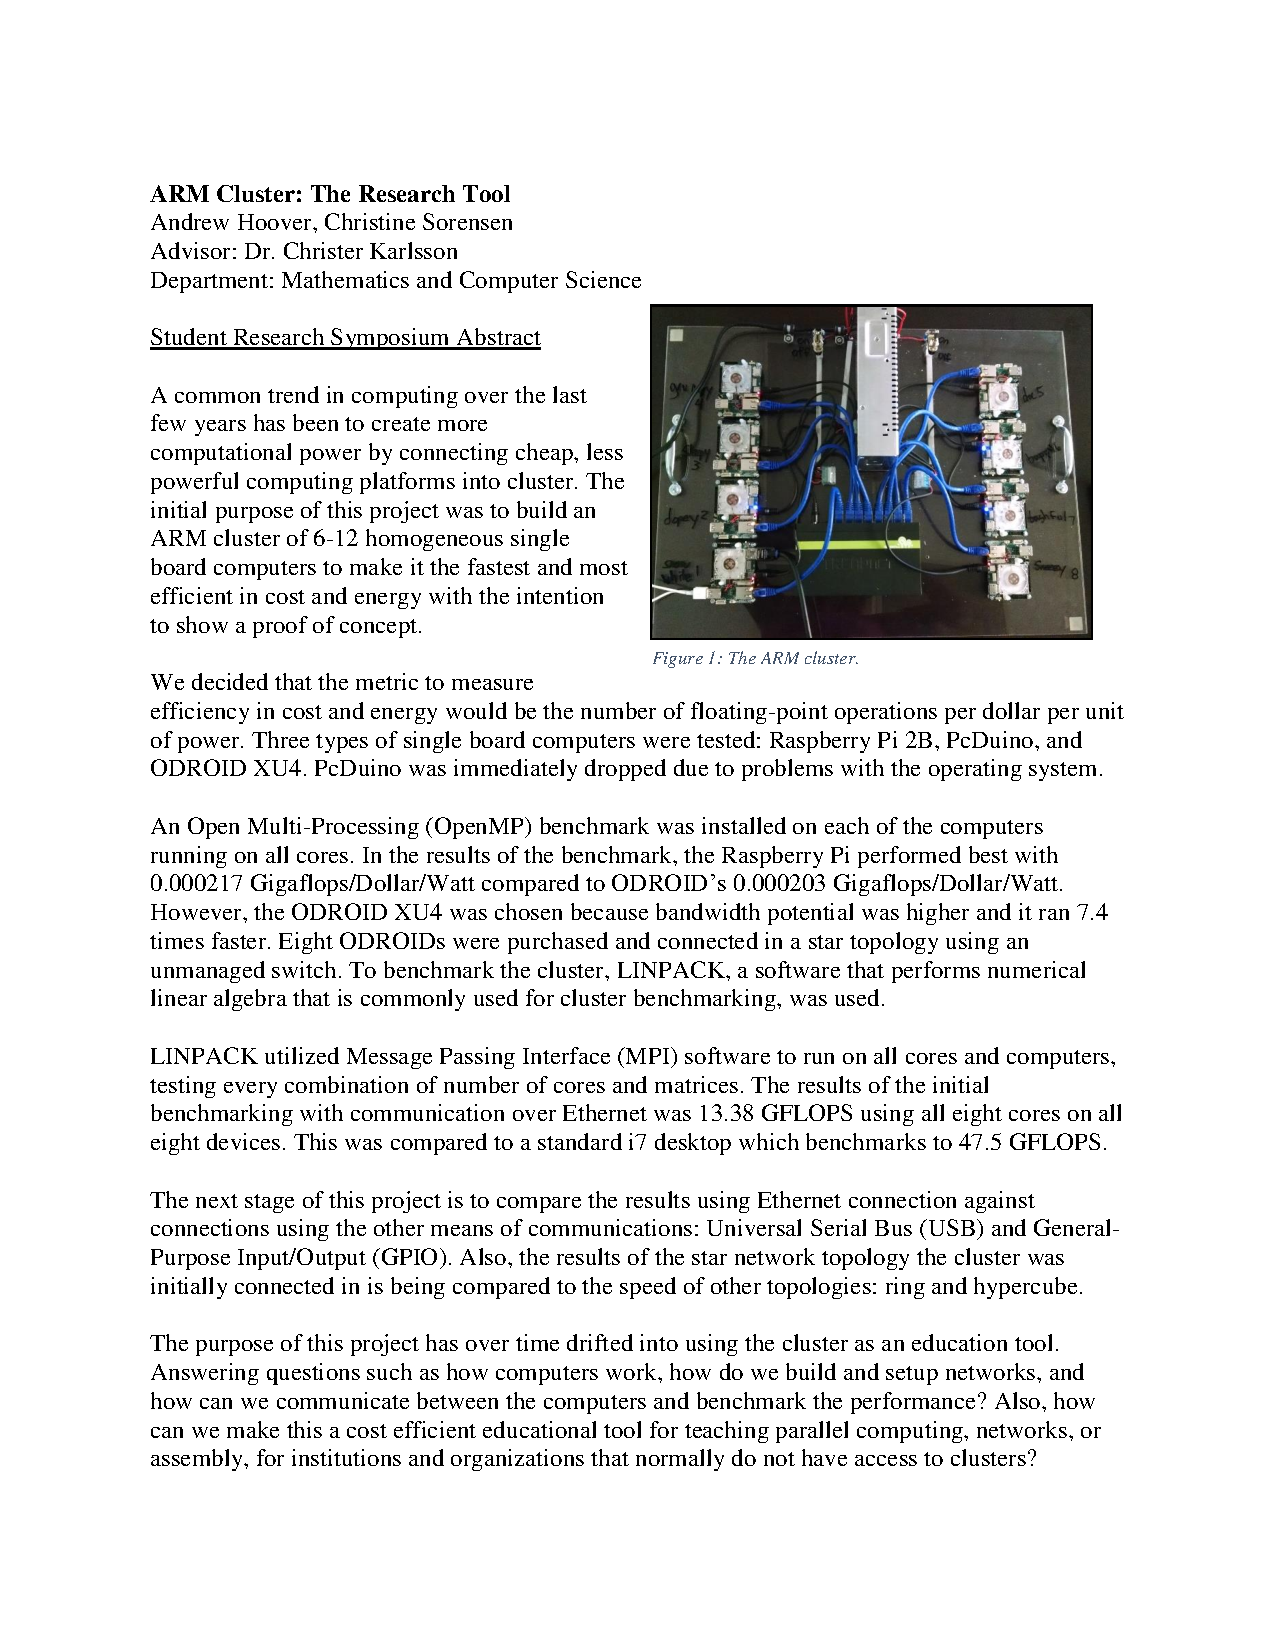
\includepdf[pages={1-1}]{SDSMTResearchAbstract.pdf}
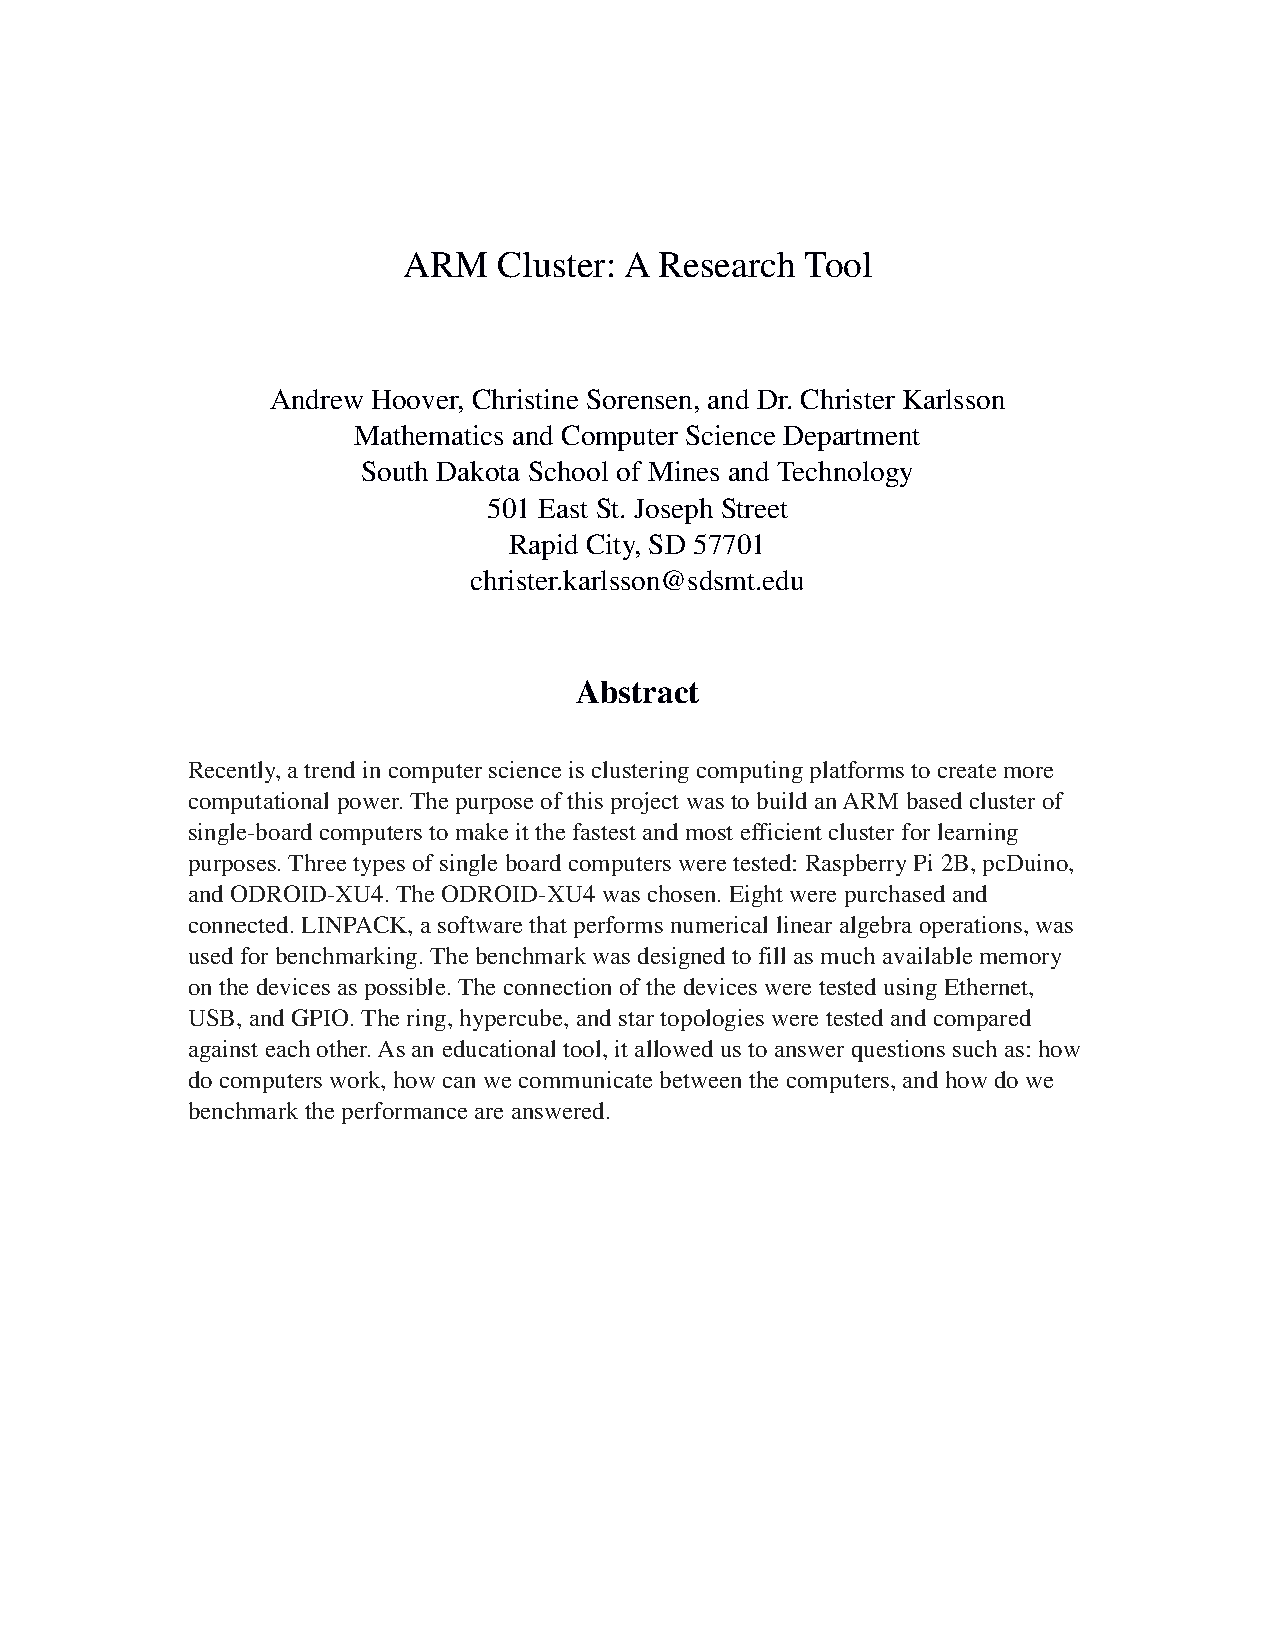
\includepdf[pages={1-9}]{MICSPaper.pdf}



\chapter{Sprint Reports}
% !TEX root = SystemTemplate.tex

%% GOT IT ALL
\section{Sprint Report \#1}

\subsection*{Overview}

\subsection*{Deliverables}
\begin{itemize}
	\item Mission Statement
	\item User Stories
	\item Number Generating Code
	\item Benchmark Code
	\item Benchmark Log
	\item Signed Software Contract
	\item Updated Design Document
\end{itemize}

\subsection*{Work for this sprint included:}
\begin{itemize}
	\item Wrote Mission Statement and Elevator Speech
	\item Drew up Software Contract
	\item Wrote user stories
	\item Obtained ODroid 4xU, Raspberry Pi 2B, and PcDuino 8 single-board computers
	\item Wrote number generating code
	\item Wrote benchmark code that ran addition, multiplication, division, and sine floating point operations
	\item Added OpenMP to run the benchmark code on all cores
	\item Ran the code each of the single-board computers
	\item Logged times
	\item Calculated the GFlops
	\item Calculated the GFlops/Dollar/Watts
	\item Determined best computer
\end{itemize}

\subsection*{Work that is carried over into Sprint 2 is as follows:}
\begin{itemize}
	\item Using the benchmark results to determine which computer to use
	\item Order more of the computers that proved best from Sprint 1 and maintain the given budget of \$1,200
	\item Find a topology that best fits the cluster
\end{itemize}

\subsection*{Backlog}
\begin{itemize}
	\item Decide on a computer based on the results of the benchmarking
	\item Calculate prices on supplies and computers while maintaining below the budget
	\item Ordering said supplies and computers
	\item Build the cluster to perform floating-point operations
	\item Benchmark the cluster
	\item Experiment with different connections
	\item Create a new mode of communication
\end{itemize}

\section{Sprint Report \#2}

\subsection*{Deliverables}
\begin{itemize}
	\item Budget
	\item Harware Tests
	\item Switch Benchmark
	\item Ethernet Benchmard
	\item USB to Ethernet
	\item MPI Code
	\item Message-Passing Protocol Design
	\item Updated Design Document
\end{itemize}

\subsection*{Overview}
During this sprint, our team first decided to use the ODROID devices instead of Raspberry PIs based on our findings from sprint one. We roughly planned out our budget for ethernet cables, the switch, varius USB cables, power strips, and the devices themselves and extra memory for them. At this stage, we did not chose exactly what we would buy, but we narrowed our budget enough to know that the number of devices we could have without going over the limit set by our sponser was eight. Dr. Karlsson then ordered seven more ODroids, an eight port switch, eight ethernet cables, and one USB to RJ45 device to benchmark USB to ethernet speeds. We encountered an issue where the order was backordered, and we did not receive the devices until over two weeks laters. Once we did get them, we benchmarked the speed over ethernet between two devices through the switch, and the speed when one device was using a USB to RJ45 to connect to the switch. We also attempted to benchmark the direct connection between RJ45 on one device connected directly to the ethernet of another device, but found that we would need a crossover cable. We concluded our sprint by setting up all eight devices by installing MPI and giving them static IP addresses on the network over the switch. \newline \newline Dr. Karlsson as been informed of a research synposium and has suggested our team take part of it. We are adding this to our goals for Senior Design to take part in that.

\subsection*{Work for this sprint included:}

\subsubsection*{Andrew Hoover}
\begin{itemize}
	\item Benchmarked:
		\begin{itemize}
			\item Switch
			\item Ethernet
			\item USB to Ethernet
		\end{itemize}
	\item Tested hardware
	\item Tested MPI code on ODROIDs
\end{itemize}

\subsubsection*{Samantha Krantz}
\begin{itemize}
	\item Researched supplies
	\item Finialized budget
	\item Researched patents and other clusters
\end{itemize}

\subsubsection*{Christine Sorensen}
\begin{itemize}
	\item Designed message-passing protocol
	\item Sampled MPI code
	\item Updated Design Document
	\item Sprint report document
\end{itemize}

\subsection*{Work that is carried over into Sprint 3 is as follows:}
\begin{itemize}
	\item Design the cluster
	\item Build the cluster
	\item Benchmark cluster
	\item Test message-passing using the other pins and ports
\end{itemize}

\subsection*{Backlog}
\begin{itemize}
	\item Build the cluster to perform floating-point operations
	\item Benchmark the cluster
	\item Experiment with different connections
	\item Create a new mode of communication
\end{itemize}

\subsection*{Goals}
\begin{itemize}
	\item Design Fair
	\item Research Symposium
\end{itemize}

\section{Sprint Report \#3}

\subsection*{Deliverables}
\begin{itemize}
	\item Built cluster
	\item MPI code
	\item Mounted home directory
	\item Shutdown script
	\item Mounting script
	\item LINPACK and ATLAS installed on ODROIDs
	\item MPI installed on ODROIDs
	\item Hostnames
	\item Fixed IP Addresses
	\item SSH configuration
\end{itemize}

\subsection{Overview}
\begin{itemize}
	\item Built cluster
	\begin{itemize}
		\item All parts for the cluster were ordered. Parts included:
		\begin{itemize}
			\item 8 ODROID XU4's
			\item Switch
			\item Power box
			\item Ethernet cables
			\item Acrylic board
			\item Accessories, such as handles and power switches
		\end{itemize}
		\item The ODROIDs, switch and power box were mounted onto the acrylic board. ODROIDs were connected to the switch and the power box.
	\end{itemize}
	\item Set up cluster
	\begin{itemize}
		\item Fixed IP addresses to each ODROID
		\item Assigned a hostname to each ODROID
		\item Configured cluster network
		\item NFS share
		\item Configured sudo
		\item Set-up ssh between ODROIDS
	\end{itemize}
	\item Benchmarked cluster
	\begin{itemize}
		\item Installed LINPACK
		\item Wrote MPI code to run on the cluster
		\item Ran the MPI code with LINPACK on the cluster
		\item Gathered data
	\end{itemize}
	\item Setbacks
	\begin{itemize}
		\item Backorder
		\begin{itemize}
			\item The remaining ODROIDs were backordered, delaying to assembling of the cluster.
		\end{itemize}	
		\item Broken ODROIDs
		\begin{itemize}
			\item Two of the ODROIDs needed to be replaced. It was believed that the two ODROIDs were placed on the power supply without covering which exposed the soldering on the bottom to sepatate it from the metal which might have crossed circuits causing the ODROIDs to not power up. Ordering the new ODROIDs put us behind in our timeline.
		\end{itemize}
		\item Installing LINPACK
		\begin{itemize}
			\item The installation of LINPACK was complicated and prompted issues. It took longer than expected to complete.
		\end{itemize}
	\end{itemize}
\end{itemize}

\subsection*{Work for this sprint included:}
\subsubsection*{Andrew Hoover}
\begin{itemize}
	\item Installed LINPACK and ATLAS
	\item Assembled cluster
	\item Replaced broken ODROIDS
	\item Fixed IP address on the ODROIDS
	\item Connected all ODROIDS over network
	\item Accessed the internet through the ODROIDS
	\item Mounted home directory of Snow White on the other ODROIDS
	\item Wrote script to shut down all ODROIDs
	\item Wrote script to run LINPACK on ODROIDs for specified number of processes
	\item Removed the sudo password
	\item Wrote script to change network configuration to all access to the internet or local network
	\item Assembled cluster
	\item Debugged boot-up error
	\item Benchmarked cluster using LINPACK and MPI code
\end{itemize}

\subsubsection*{Samantha Kranstz}
\begin{itemize}
	\item Created client presentation 
	\item Assembled cluster
	\item Debugged boot-up error
	\item Benchmarked cluster using LINPACK and MPI code
	\item Researched patents
\end{itemize}

\subsubsection*{Christine Sorensen}
\begin{itemize}
	\item Assigned hostnames to each of the ODROIDs
	\item Configured ssh on ODROIDs
	\item Replaced broken ODROIDs
	\item Wrote MPI code to run on all cores of the clusters
	\item Updated design documentation
	\item Wrote script to mount home directory of Snow White onto all ODROIDS at once
	\item Added ODROID's hostnames to the others' known hosts list
	\item Wrote sprint report 
	\item Assembled cluster
	\item Debugged boot-up error
	\item Benchmarked cluster using LINPACK and MPI code
\end{itemize}

\subsection*{Work that is carried over into Sprint 4 is as follows:}
\begin{itemize}
	\item Research new methods of connection
	\item Take action on these new methods
	\item Benchmark
	\item Complete abstract for research symposium
\end{itemize}

\subsection*{Backlog}
\begin{itemize}
	\item Research new connection methods
	\item Benchmark the cluster
	\item Experiment with different topologies
	\item Create a new mode of communication
	\item Design documentation
	\item Research symposium
	\begin{itemize}
		\item Complete abstract
	\end{itemize}
	\item Design Fair
\end{itemize}

\section{Sprint Report \#4}

\section{Sprint Report \#5}

\section{Sprint Report \#6}

\chapter{Industrial Experience and Resumes}
%OLD
% !TEX root = SystemTemplate.tex


\section{Resumes}

%%Your resumes are included here.  See the source file (industrial.tex) and uncomment the PDF includes to see how this works.  If your resume is written in \LaTeX\ then you can just insert the \LaTeX\ source code.

%    \includepdf[pages={1}]{report.pdf}  %% example of limited page include

     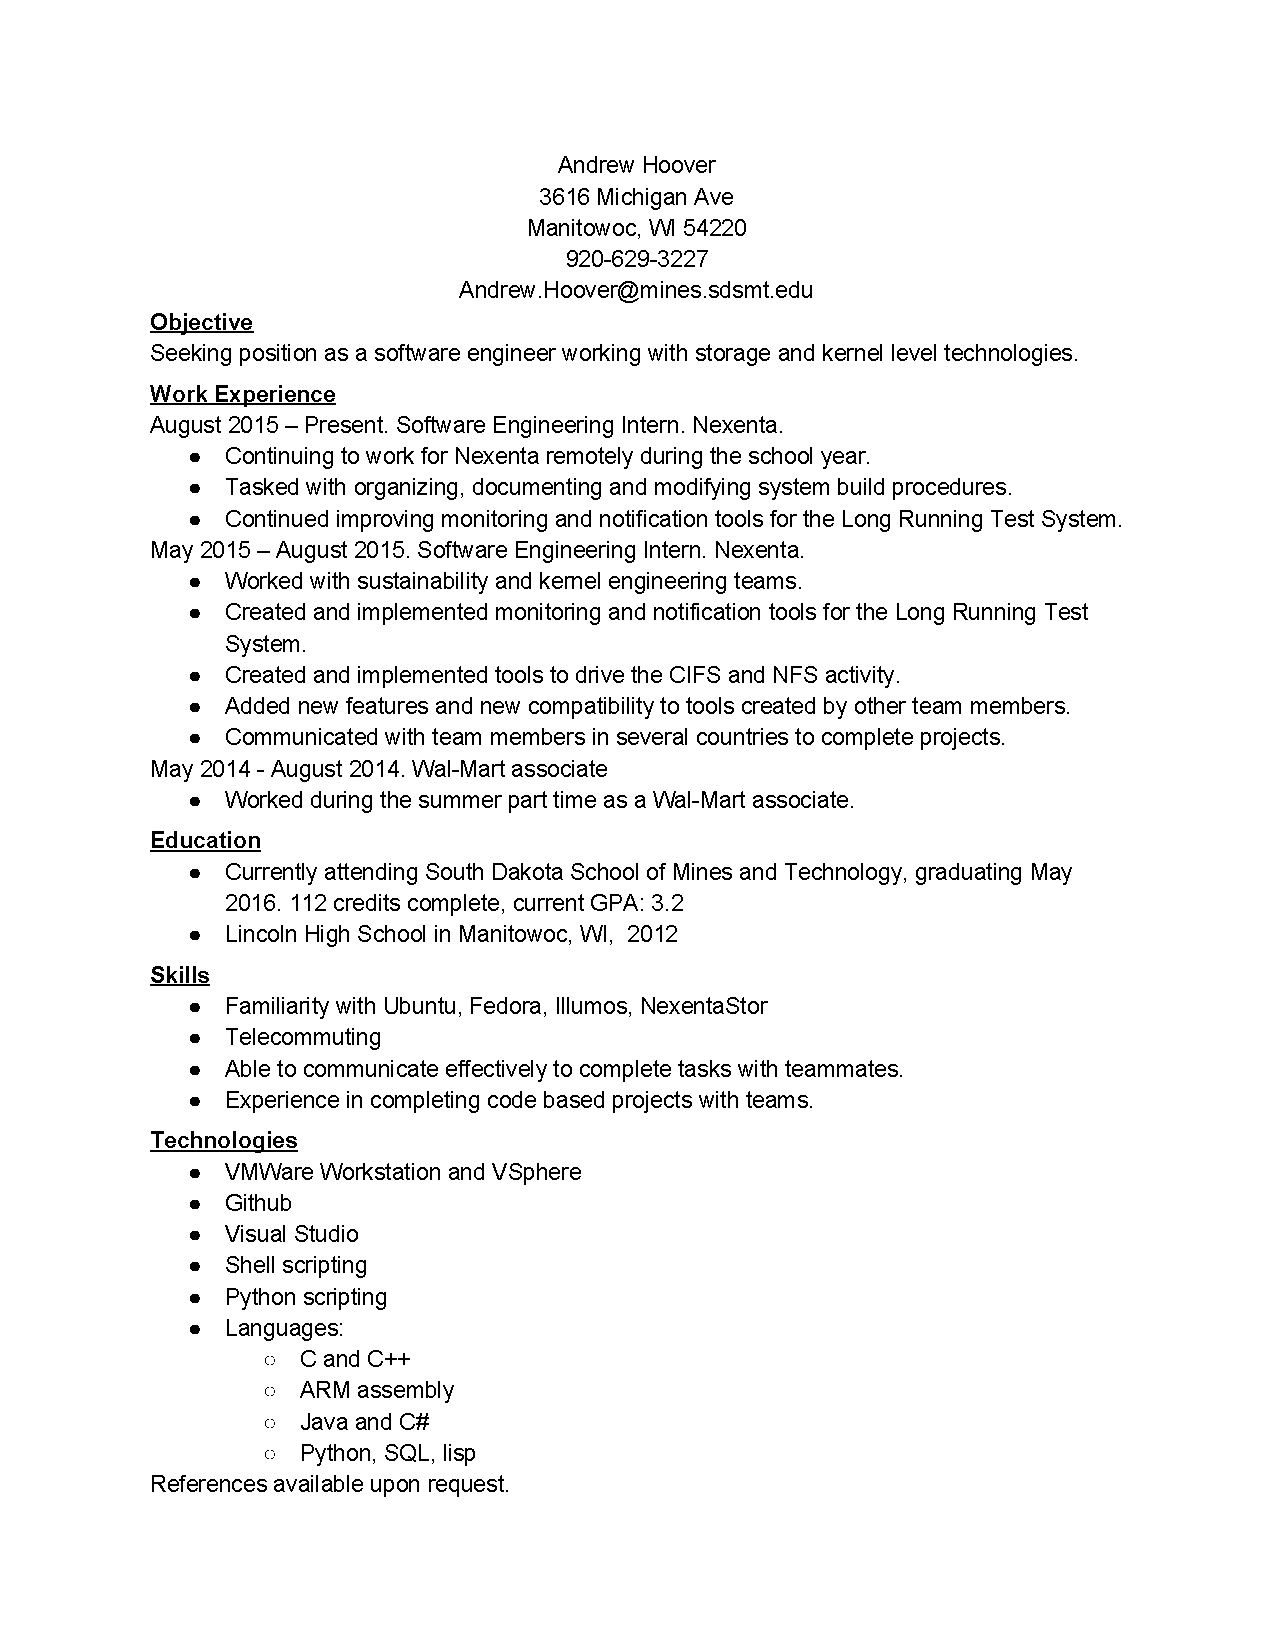
\includepdf{HooverResume.pdf}
     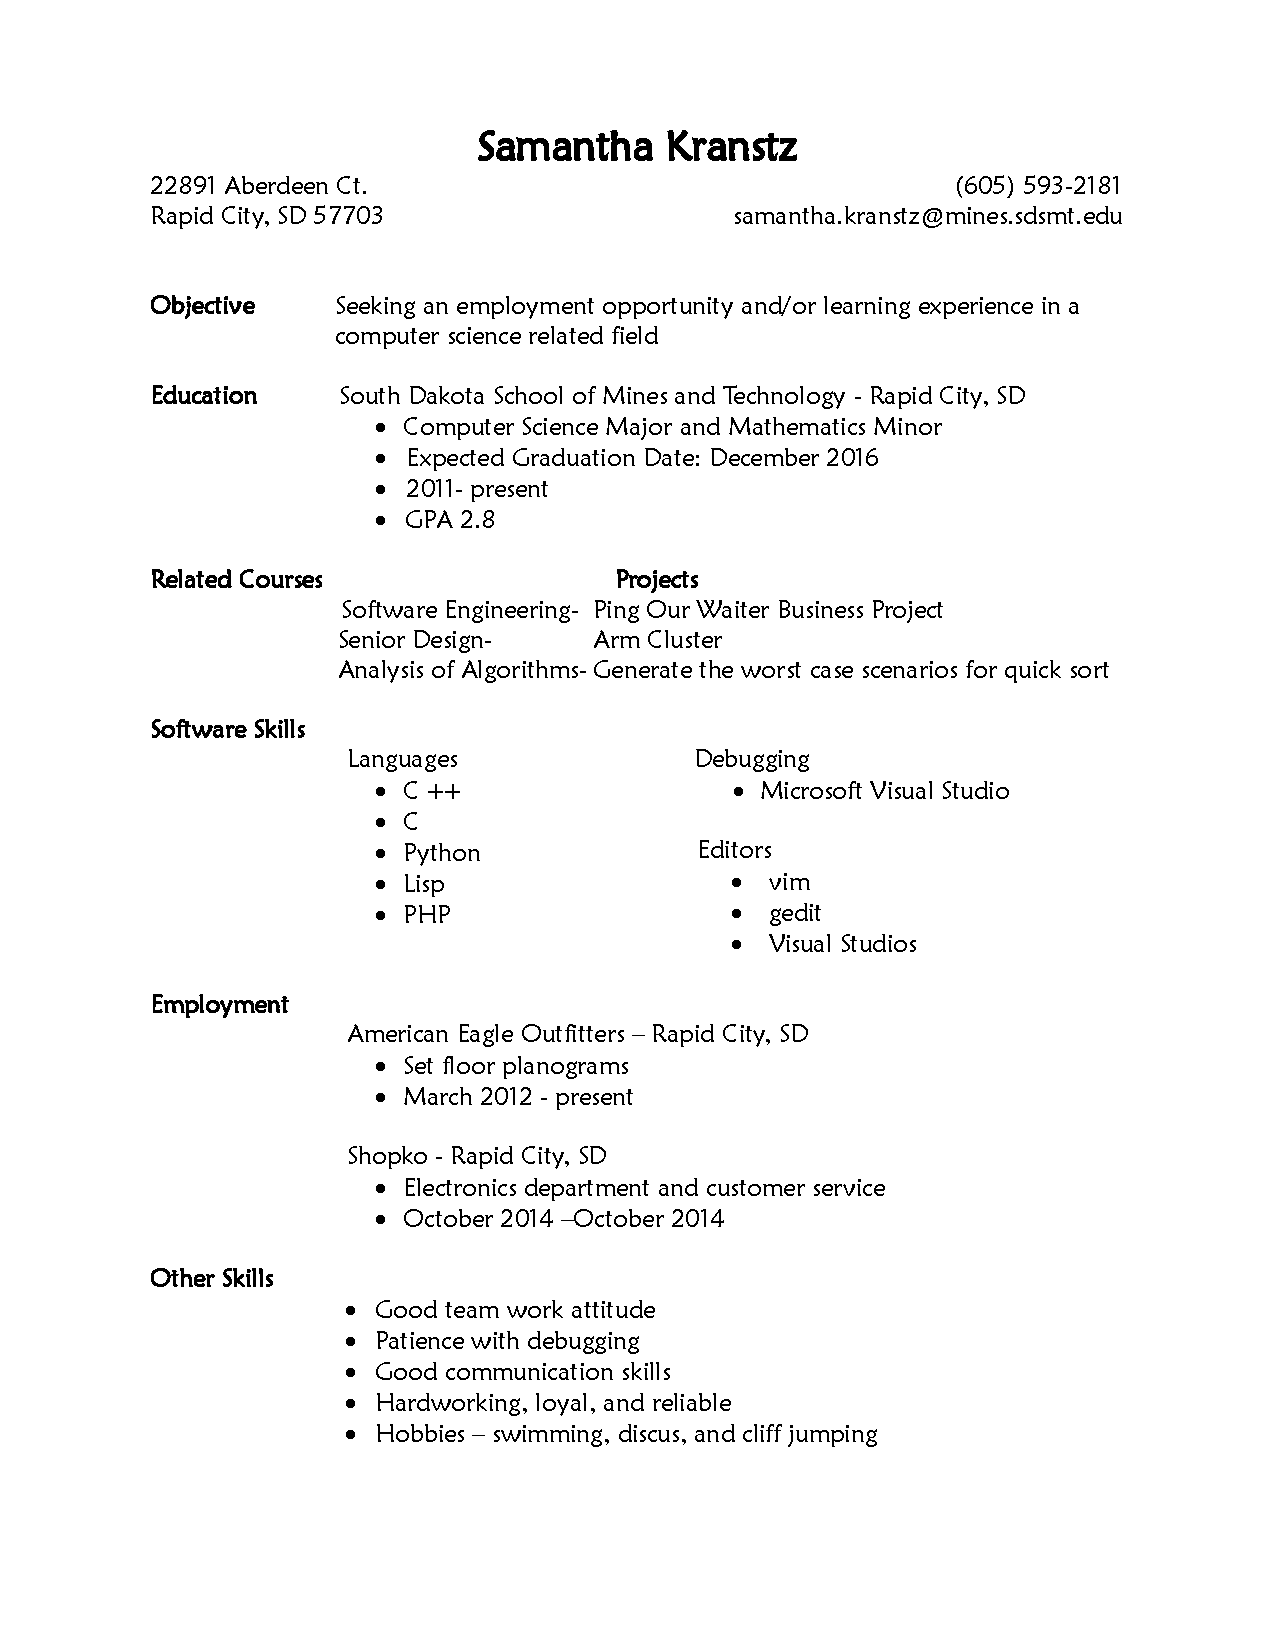
\includepdf{KranstzResume.pdf}
     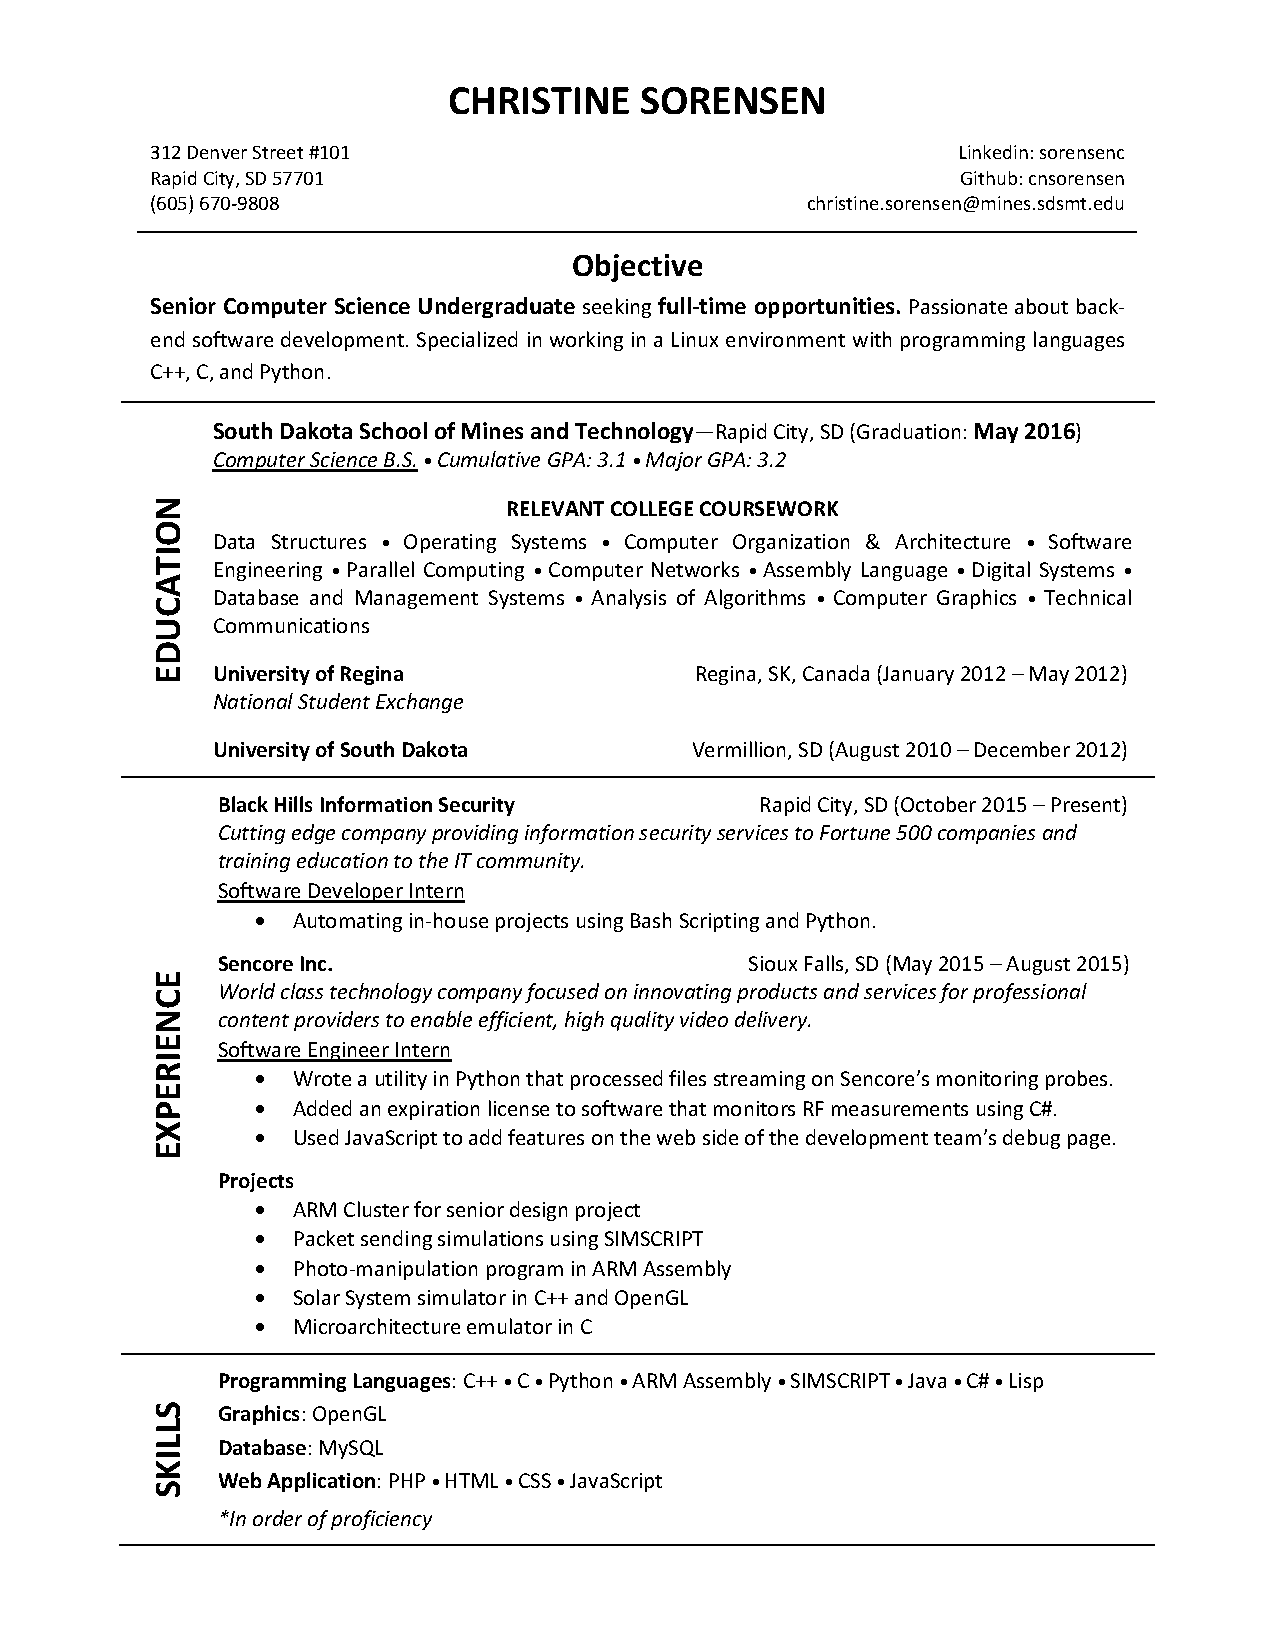
\includepdf{SorensenResume.pdf}

%%We need to figure this out eventually - cns
%%\section{ABET:  Industrial Experience Reports}

%%\subsection{Name1}

% \includepdf{name1.pdf}

%%\subsection{Name2}

% \includepdf{name2.pdf}

%%\subsection{Name3}

% \includepdf{name3.pdf}




\chapter{Acknowledgment}
\label{SpecialThanks}  
Thanks  

%%\chapter{Supporting Materials}
%%
This document will contain several appendices used as a way to separate out major 
component details, logic details, or tables of information.  Use of this structure 
will help keep the document clean, readable, and organized. 



% chapters in backmatter don't have numbers, but they appear in the
% table of contents, and are numbered BM-X where X is the page number
% relative to where the backmatter begins.
\backmatter

%% Example
%\chapter{Course Syllabus}
%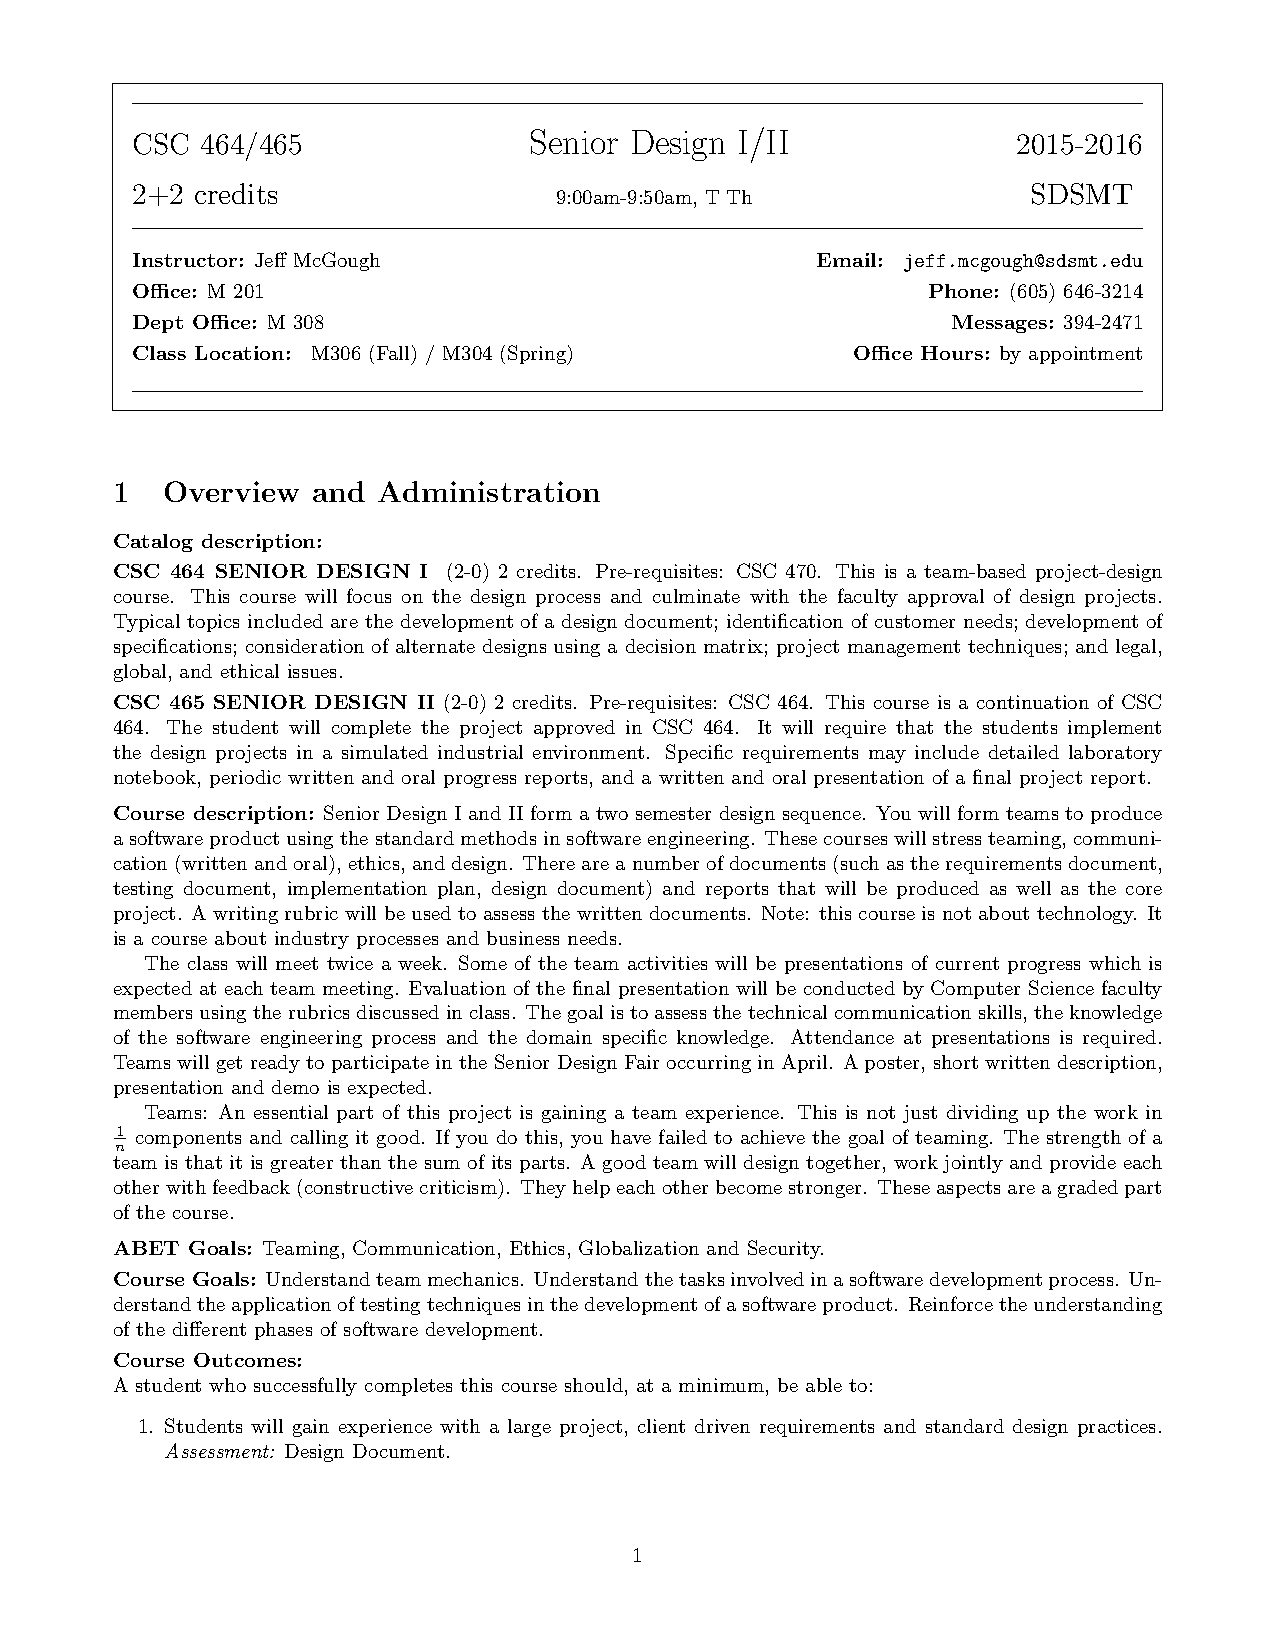
\includepdf[pages={1-17}]{syllabus.pdf}





\end{document}
